\documentclass[12pt, a4paper]{article}

\usepackage{array}
\usepackage[portuguese]{babel}
\usepackage{float}
\usepackage[a4paper, margin=2cm]{geometry}
\usepackage{graphicx}
\usepackage{hyperref}
\usepackage{pdfpages}
\usepackage{setspace}

\title{\textbf{Interface Pessoa-Máquina \\ \large Trabalho Prático -- Fase II}}
\date{4 de maio de 2025}
\author{Grupo 12 \\ \\
    \url{https://www.figma.com/design/Ps4VLCPz66bKq5p2ypzrDR/Projeto-IPM} \\ \\
    \url{https://github.com/UMinho-ENGINF-IPM/trabalho-pr-tico-gp25_12}}

\begin{document}

\begin{center}
    
\includegraphics[width=0.25\textwidth]{res/cover/school-of-engineering.eps}
\end{center}

{\let\newpage\relax\maketitle}
\maketitle
\thispagestyle{empty}

\chardef\_=`_
\onehalfspacing
\setlength{\parskip}{\baselineskip}
\setlength{\intextsep}{2\baselineskip}
\setlength\belowcaptionskip{-\baselineskip}
\setlength{\parindent}{0pt}
\def\arraystretch{1.5}

\begin{center}
    \begin{tabular}{>{\centering}p{0.25\textwidth}
                    >{\centering}p{0.25\textwidth}
                    >{\centering\arraybackslash}p{0.25\textwidth}}
        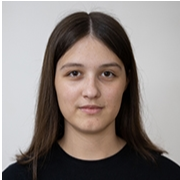
\includegraphics[width=3.5cm]{res/cover/A104437.png} &
        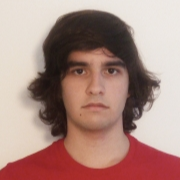
\includegraphics[width=3.5cm]{res/cover/A104348.png} &
        
\includegraphics[width=3.5cm]{res/cover/A104263.png}  \\

        Ana Oliveira & Humberto Gomes & Inês Marques \\
        A104437      & A104348        & A104263
    \end{tabular}

    \begin{tabular}{>{\centering}p{0.25\textwidth}
                    >{\centering\arraybackslash}p{0.25\textwidth}}
        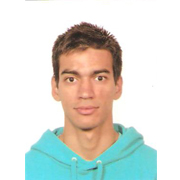
\includegraphics[width=3.5cm]{res/cover/A76350.jpg} &
        
\includegraphics[width=3.5cm]{res/cover/A104179.png} \\

        Rafael Vilas Boas & Sara Lopes \\
        A76350            & A104179
    \end{tabular}
\end{center}

\begin{abstract}
    \noindent
    No âmbito da segunda fase deste trabalho prático, foi implementada, com base em modelação
    prévia, uma interface de utilizador de um sistema para a gestão de horários de um curso
    universitário, utilizado tanto pelos alunos como pelo diretor de curso. Neste documento,
    apresenta-se a interface implementada em Vue \cite{vue} (e outras tecnologias) e o seu processo
    de implementação, bem como algumas correções feitas ao modelo da interface. Por falta de tempo,
    não foi possível fazer testes da aplicação com utilizadores reais, não sendo possível fazer uma
    reflexão muito aprofundada sobre a qualidade do produto final. No entanto, consideramos que a
    aplicação desenvolvida cumpriu os requisitos pedidos.
\end{abstract}

\section{Objetivos}

O objetivo do trabalho prático proposto na Unidade Curricular de Interface Pessoa-Máquina é a
modelação e o desenvolvimento de uma aplicação Web para para a gestão de horários de um curso
universitário, utilizada tanto pelos alunos como pelo diretor de curso. Em particular, deseja-se que
a aplicação permita aos alunos consultar o seu horário e fazer pedidos de troca de turno ao diretor
de curso, e que o diretor de curso possa manualmente colocar alunos em turnos (para resolver
limitações do algoritmo de colocação e aceder a pedidos de alunos) e aceder a pedidos de professores
para mudança de turnos para salas maiores. Para mais detalhes, o enunciado do trabalho prático pode
ser consultado nos anexos deste relatório. Idealmente, a aplicação deve ajudar o utilizador a não
cometer erros, como colocar alunos em turnos que originem sobreposições de horário.

Na primeira fase deste trabalho, fez-se a modelação da aplicação em Figma \cite{figma}, e nesta
fase, procurou-se implementar a interface modelada em Vue \cite{vue}. Também se realizaram algumas
alterações ao modelo, a corrigir alguns aspetos que se acharam relevantes.

\section{Alterações ao Modelo da Interface}

Na fase anterior deste trabalho prático, construiu-se, em Figma \cite{figma}, um modelo da interface
a implementar. Apesar de uma boa avaliação nesta fase, a docência da UC de Interface Pessoa-Máquina
reparou em alguns aspetos que podiam ser melhorados. Nesta secção, apresentam-se as mudanças que
foram feitas ao modelo da interface devido tanto aos comentários dos docentes como a outros aspetos
que o nosso grupo de trabalho se apercebeu que podiam ser melhorados.

Em primeiro lugar, a página ``Iniciar Sessão'' não é ideal para a prevenção de erros: é possível que
o utilizador submeta parcialmente as suas credenciais (apenas o seu endereço eletrónico ou apenas a
sua palavra-passe), e o sistema reagirá com um erro. Para prevenir este erro, deve ser impossível
que um utilizador submeta as suas credenciais até as escrever todas. Logo, na nova versão do modelo
da interface, o botão de submissão de credenciais encontra-se desativado até o utilizador escrever
tanto o seu endereço eletrónico como a sua palavra-passe, como mostra a figura abaixo:

\begin{figure}[H]
    \centering
    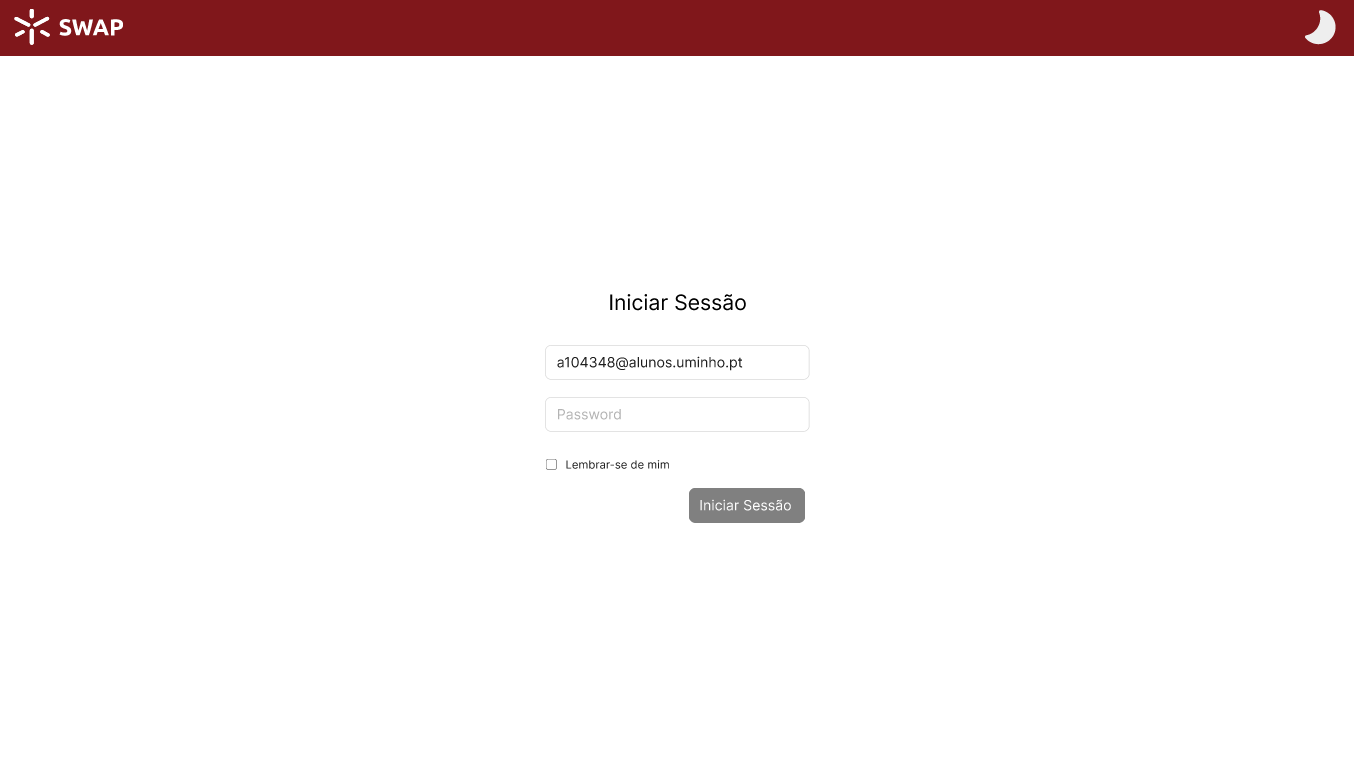
\includegraphics[width=0.8\textwidth]{res/prototype/iniciar-sessao-botao-desativado-email.png}
    \caption{Captura de ecrã do protótipo da página ``Iniciar Sessão'' com botão desativado.}
    \label{iniciar-sessao-botao-desativado-email}
\end{figure}


É importante que o utilizador saiba por que este botão se encontra desativado, pelo que, tal como
foi feito em outros botões na interface, uma \emph{tooltip} foi utilizada para justificar por que
não é possível interagir com o botão:

\begin{figure}[H]
    \centering
    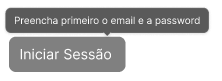
\includegraphics[width=0.3\textwidth]{res/prototype/inicar-sessao-tooltip-botao-desativado.png}
    \caption{\emph{Tooltip} sobre o botao de início de sessão desativado.}
    \label{inicar-sessao-tooltip-botao-desativado}
\end{figure}

Ademais, na página ``Resolver Problemas'', o título da página foi removido, e substituído por uma
barra de pesquisa. Em primeiro lugar, o título da página não era necessário, visto que o utilizador
já sabe em que página se encontra olhando para a hiperligação realçada na barra de navegação.
Depois, o espaço que se ganha na barra lateral com a remoção deste título pode ser usado uma barra
de pesquisa, um elemento muito útil para procurar alunos em grandes listas de problemas (o cenário 1
aponta para 45 alunos sem turnos atribuídos).

\begin{figure}[H]
    \centering
    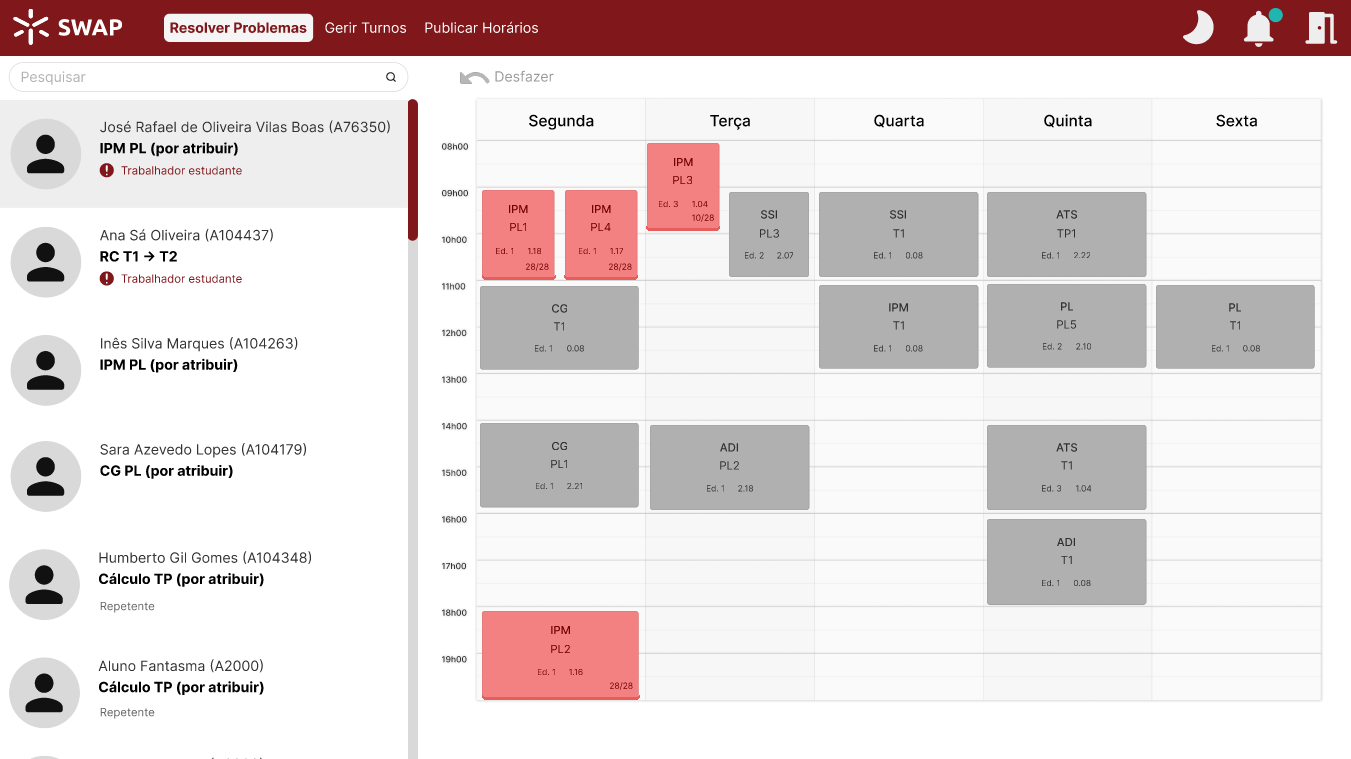
\includegraphics[width=0.8\textwidth]{res/prototype/resolver-problemas-revisto.png}
    \caption{Captura de ecrã do protótipo da página ``Resolver Problemas''.}
    \label{resolver-problemas-revisto}
\end{figure}

De seguida, uma sugestão da docência de Interface Pessoa-Máquina foi a eliminação da página
``Publicar Horários'', sendo estes atualizados sempre que o diretor de curso faz uma alteração. No
entanto, não consideramos esta solução viável, visto que o diretor de curso pode desejar colocar os
horários dos alunos em estados intermédios sem que estes os vejam. Por exemplo, pode desejar remover
vários alunos dos seus turnos, para os adicionar a outros turnos da mesma UC, assim, por exemplo,
abrindo vagas em turnos mais procurados. No entanto, reparou-se que é importante realçar quando as
mudanças feitas pelo diretor de curso ainda não são públicas. Por este motivo, tal como foi feito
para o ícone de notificações, quando há alterações de horário por publicar, um pequeno círculo é
adicionado ao canto superior direito da hiperligação para a página ``Publicar Horários'', como
mostra a figura abaixo:

\begin{figure}[H]
    \centering
    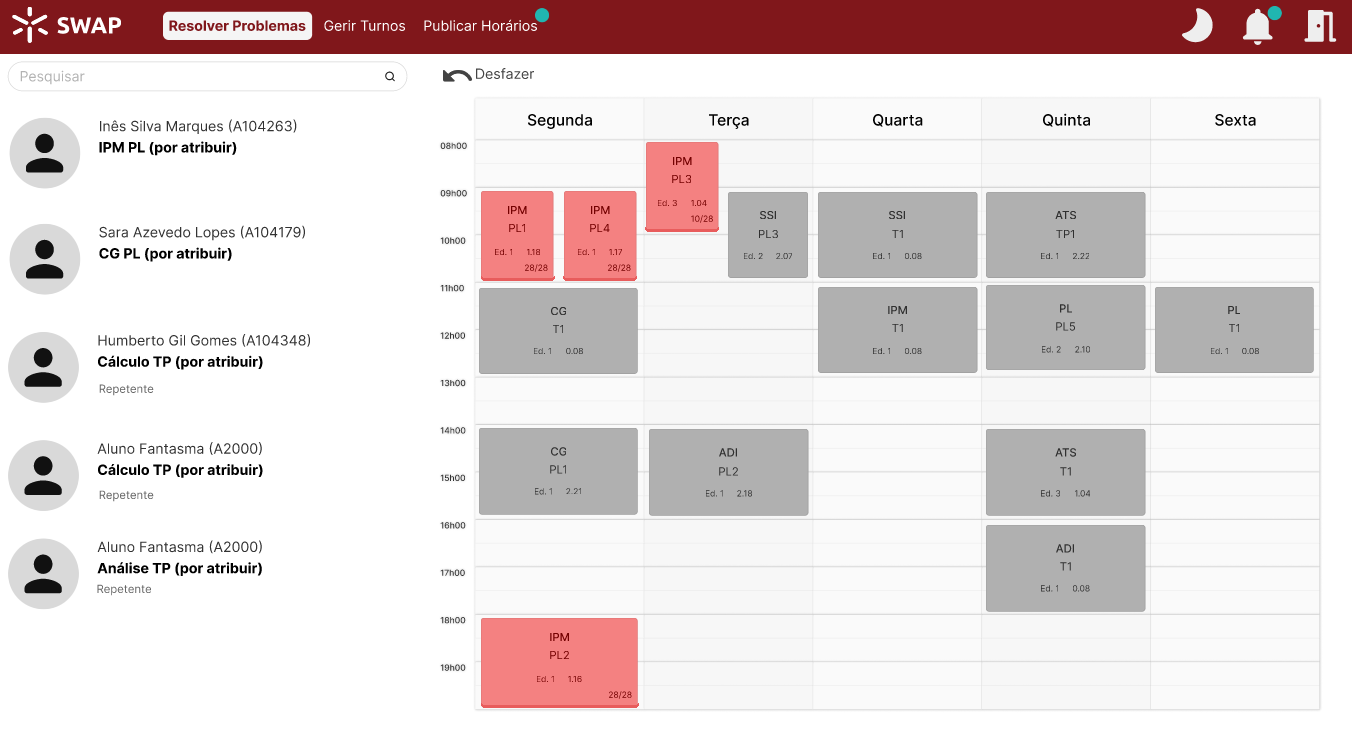
\includegraphics[width=0.8\textwidth]{res/prototype/mudancas-feitas-publicar-horario.png}
    \caption{
        \onehalfspacing
        Captura da barra de navegação com realce na hiperligação para a página
        ``Publicar Horários''.
    }
    \label{mudancas-feitas-publicar-horario}
\end{figure}

No entanto, partindo da solução de não ser necessário publicar os horários, fez-se não ser
necessário, na página ``Gerir Turno'', guardar as alterações feitas a um turno: estas são guardadas
à medida que o utilizador as faz. Logo, o botão ``Guardar'' foi substituído por um botão ``Voltar''.
Na mesma página, desfazer uma alteração deixou de ser feito através de uma \emph{toast} que aparecia
sempre que uma alteração era feita, e sim por um botão ``Desfazer'', de forma consistente com a
página ``Resolver Problemas'':

\begin{figure}[H]
    \centering
    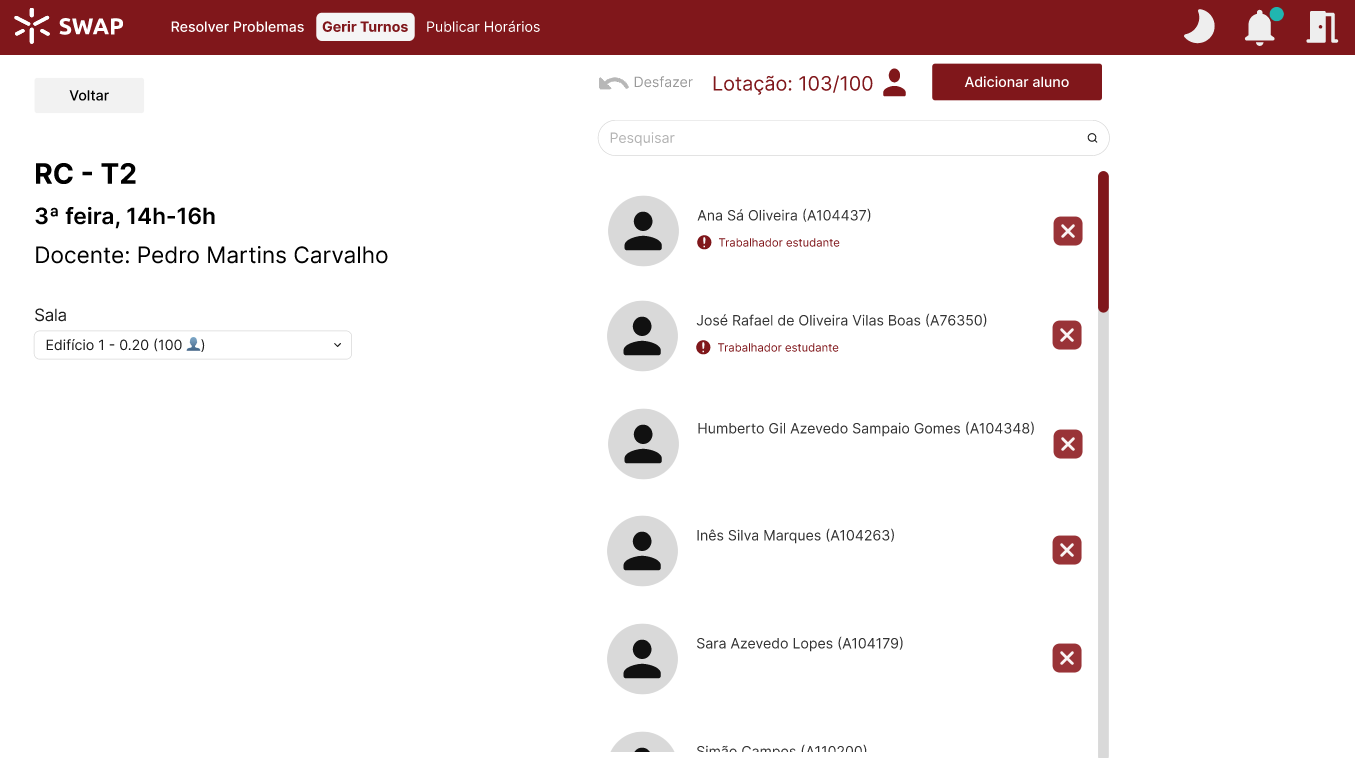
\includegraphics[width=0.8\textwidth]{res/prototype/gerir-turnos-revisto.png}
    \caption{Captura de ecrã do protótipo da página ``Gerir Turnos''.}
    \label{gerir-turnos-revisto}
\end{figure}

Na página ``Notificações'', o botão para alternar entre visualizar todas as notificações ou apenas
as não lidas foi removido, visto que as mesmas já se encontram ordenadas por este critério:

\begin{figure}[H]
    \centering
    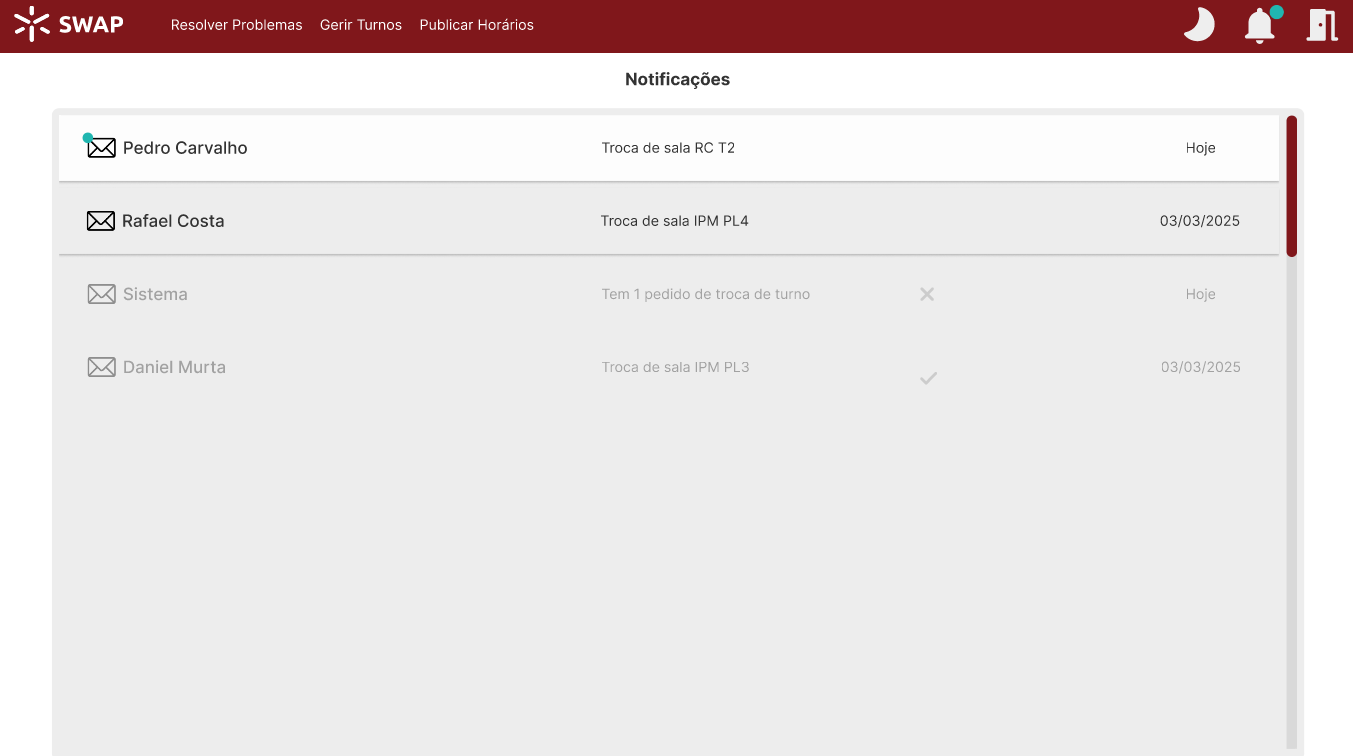
\includegraphics[width=0.8\textwidth]{res/prototype/notificacoes-diretor-revisto.png}
    \caption{Captura de ecrã do protótipo da página ``Notificações'' do diretor de curso.}
    \label{notificacoes-diretor-revisto}
\end{figure}

Por último, também se seguiu a sugestão da equipa docente de mostrar o estado dos pedidos nas
páginas ``Histórico de Pedidos'' e ``Notificações do Diretor de Curso''. Abaixo, apresenta-se, como
exemplo, o modelo da página ``Histórico de Pedidos''. Apesar do uso de linguagem iconográfica, tal
como no resto da aplicação, os ícones apresentados têm todos \emph{tooltips}, que são ativadas após
o cursor os sobrevoar por alguns segundos:

\begin{figure}[H]
    \centering
    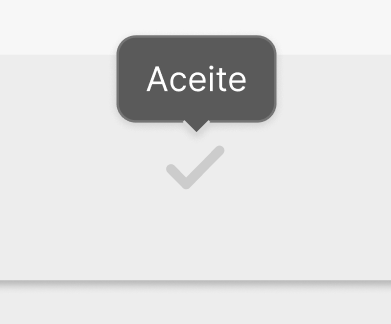
\includegraphics[width=0.2\textwidth]{res/prototype/estado-pedido-tooltip.png}
    \caption{\emph{Tooltip} sobre o estado de um pedido.}
    \label{estado-pedido-tooltip}
\end{figure}

\section{Componentes Implementados}

O primeiro passo no processo de implementação da interface foi a identificação de componentes e
respetiva implementação. Foram identificados como componentes \emph{widgets} comuns (botões, campos
de texto, \ldots) e outros elementos presentes em várias páginas / várias vezes na mesma página.
Note-se que \emph{widgets} simples foram implementados como componentes (em vez de serem usados
diretamente) para haver um maior controlo sobre o estilo que é aplicado aos mesmos, e para ser
possível suportar várias variantes dos mesmos. Segue-se uma breve lista dos vários componentes
desenvolvidos:

\subsection{Alerta}

Este componente estático apresenta uma informação importante ao utilizador. É utilizado, por
exemplo, para informar o utilizador na página ``Iniciar Sessão'' que as credenciais que submeteu se
encontram incorretas, ou nos componentes ``Aluno'' e ``Problema'' que um aluno é
trabalhador-estudante, como se vê na figura \ref{problem}.

\subsection{Barra de Navegação}

Este componente está presente no topo de todas as páginas implementadas, e permite ao utilizador
rapidamente navegar para outras páginas de interesse, bem como alterar o seu tema (claro ou escuro)
e terminar sessão. Este componente, como se vê abaixo, existe em três variantes, uma para antes de
se ter iniciado sessão, uma para alunos, e outra para o diretor de curso. A barra de navegação
subdivide-se em vários subcomponentes, que não serão mencionados neste relatório, visto que apenas
existem para dividir a barra de navegação em partes mais pequenas, dando origem a código mais
modular.

\begin{figure}[H]
    \centering
    
\includegraphics[width=\textwidth]{res/components/navbar-login.png}
    
\includegraphics[width=\textwidth]{res/components/navbar-student.png}
    
\includegraphics[width=\textwidth]{res/components/navbar-director.png}
    \caption{
        \onehalfspacing
        De cima para baixo, variantes de \emph{login}, de aluno, e do diretor de curso da barra de
        navegação.
    }
    \label{navbar}
\end{figure}

\subsection{Botão}

Este componente, presente em diversas páginas da aplicação, trata-se de um \emph{widget} no qual se
pode clicar para se realizar uma ação pré-determinada. Existem várias variantes de botão (ativo, de
cancelamento, e desativado), distinguíveis pela sua cor. Adicionalmente, botões desativados podem
ter uma \emph{tooltip} a explicar por que motivo não é possível interagir com eles. Abaixo,
apresentam-se os três tipos de botão implementados:

\begin{figure}[H]
    \centering
    
\includegraphics[width=\textwidth]{res/components/button.png}
    \caption{Da esquerda para a direita, variantes de cancelamento, desativada e ativa de botões.}
    \label{button}
\end{figure}

\subsection{Botão para Desfazer}

Este componente trata-se de um botão especial, utilizado para desfazer ações nas páginas
``Resolver Problemas'' e ``Gerir Turno''. Pode ser visto na figura abaixo:

\begin{figure}[H]
    \centering
    
\includegraphics[width=3cm]{res/components/undo-button.png}
    \caption{Botão para desfazer.}
    \label{undo-button}
\end{figure}

\subsection{Capacidade}

Este componente apresenta a utilização de um turno em função da sua capacidade, sendo utilizado na
página ``Gerir Turno'', no componente ``Turno'', e no diálogo de informação sobre um turno nas
páginas ``O Meu Horário'' e ``Horário Completo''. Opcionalmente, este componente pode passar a ser
representado a vermelho caso um turno exceda a sua capacidade, como pode ser visto na figura abaixo:

\begin{figure}[H]
    \centering
    
\includegraphics[width=4cm]{res/components/capacity.png}
    \caption{Capacidade de um turno sobrelotado.}
    \label{capacity}
\end{figure}

\subsection{Campo de texto}

Este componente, presente em várias páginas da aplicação, permite ao utilizador escrever texto a ser
consumido pelo programa. Existem três variantes deste componente, para entrada de texto, para
entrada de \emph{passwords}, e uma barra de pesquisa. Na figura abaixo, podem observar-se estas três
variantes do campo de texto:

\begin{figure}[H]
    \centering
    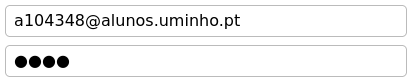
\includegraphics[width=8cm]{res/components/text-input-regular-password.png} \\
    
\includegraphics[width=8cm]{res/components/text-input-search.png}
    \caption{
        Campos de texto para entrada textual, entrada de \emph{passwords}, e barra de pesquisa.
    }
    \label{text-input}
\end{figure}

\subsection{\emph{Check box}}

Este componente permite ao utilizador definir o valor de um booleano. Destaca-se o seu uso no
componente ``Seletor de Turnos'', visível na figura \ref{shift-selector}.

\subsection{\emph{Dropdown}}

Presente apenas na página ``Gerir turno'', este componente permite ao utilizador escolher uma de
diversas opções, no caso, uma de diversas salas, como se pode ver abaixo:

\begin{figure}[H]
    \centering
    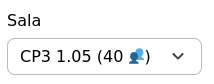
\includegraphics[width=4cm]{res/components/dropdown.png}
    \caption{\emph{Dropdown}.}
    \label{dropdown}
\end{figure}

\subsection{Estudante e Problema}

Estes dois componentes são bastante semelhantes, e permitem apresentar um estudante e um problema
(pedido de troca ou turno por atribuir), respetivamente. O componente ``Problema'' pode observar-se
abaixo:

\begin{figure}[H]
    \centering
    
\includegraphics[width=7cm]{res/components/problem.png}
    \caption{
        \onehalfspacing
        Problema de turno por atribuir. Caso apenas se apresentasse o aluno, a linha
        ``FCD T (por atribuir)'' não seria visível.
    }
    \label{problem}
\end{figure}

\subsection{Horário}

Este componente, utilizado em diversas páginas, permite apresentar um conjunto de turnos,
organizados temporalmente ao longo de uma semana, como se pode ver abaixo:

\begin{figure}[H]
    \centering
    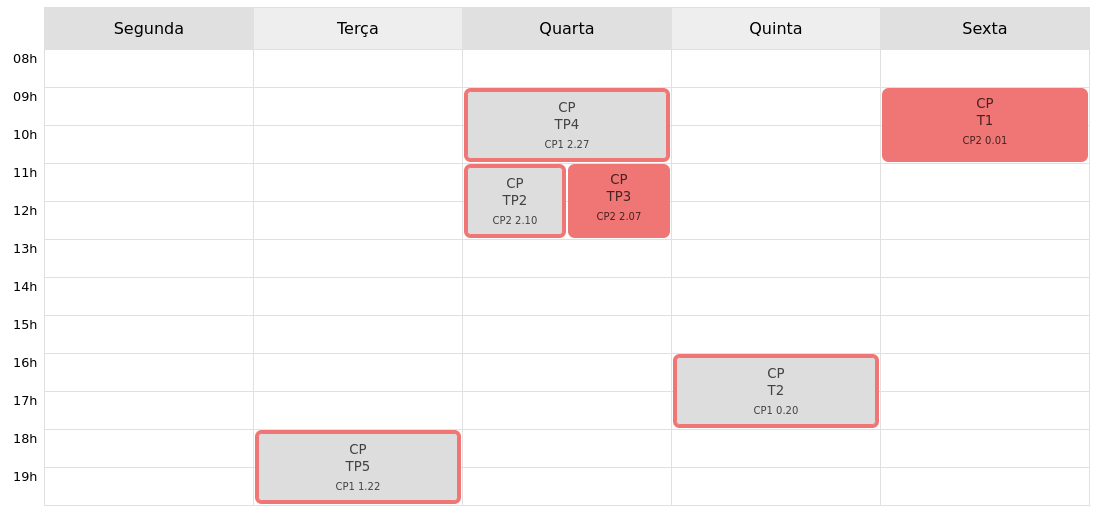
\includegraphics[width=0.45\textwidth]{res/components/schedule-1.png}
    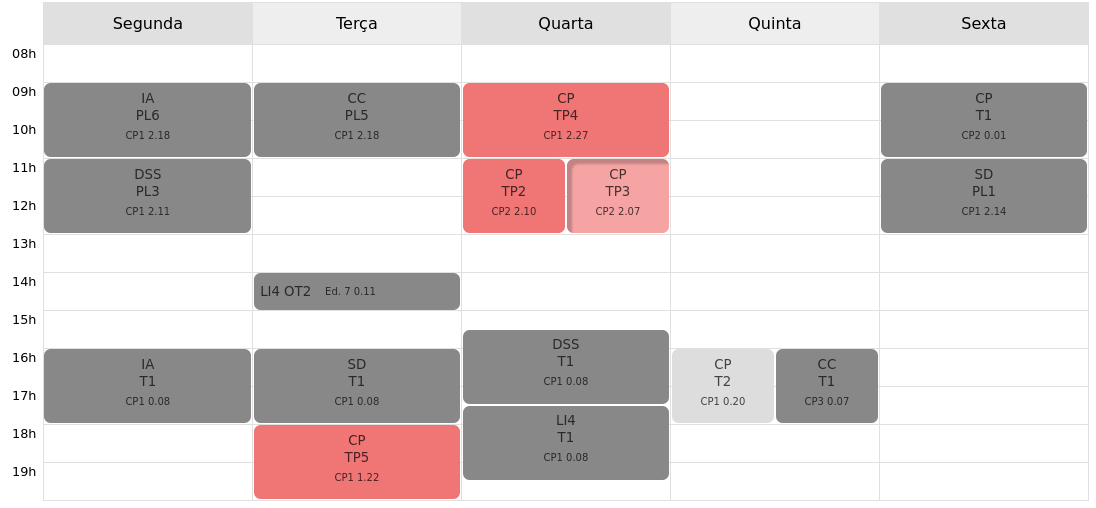
\includegraphics[width=0.45\textwidth]{res/components/schedule-2.png}
    \caption{Horários com diferentes tipos de turnos.}
    \label{schedule}
\end{figure}

\subsection{Ícone da Aplicação}

Este componente estático é usado na barra de navegação e na barra de janela do componente ``Popup''.
Pode ser visto na figura abaixo:

\begin{figure}[H]
    \centering
    
\includegraphics[width=4cm]{res/components/application-icon.png}
    \caption{Ícone da aplicação.}
    \label{application-icon}
\end{figure}

\subsection{Lista de Estudantes}

Este componente, utilizado na página ``Gerir Turno'', apresenta uma lista de estudantes, onde cada
estudante se encontra associado a um botão, que pode ser usado para o adicionar a / remover de um
turno. Este componente pode ser visto na figura abaixo:

\begin{figure}[H]
    \centering
    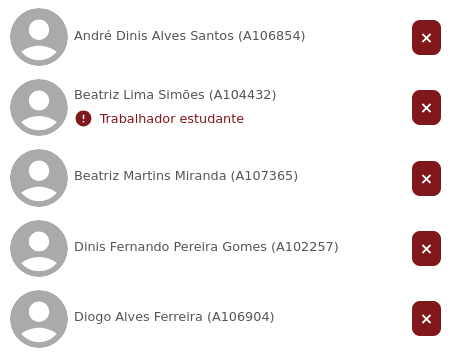
\includegraphics[width=10cm]{res/components/student-list.png}
    \caption{Lista para remoção de estudantes.}
    \label{student-list}
\end{figure}

\subsection{\emph{Popup}}

Este componente é um diálogo com uma borda de janela. Várias páginas utilizam \emph{popups}, mas
dois destes, para mostrar informação de um turno e para confirmar a troca entre dois turnos,
apresentados abaixo, foram transformados em componentes, visto que estão presentes em mais do que
uma página, no caso, ``O meu Horário'' e ``Horário Completo''.

\begin{figure}[H]
    \centering
    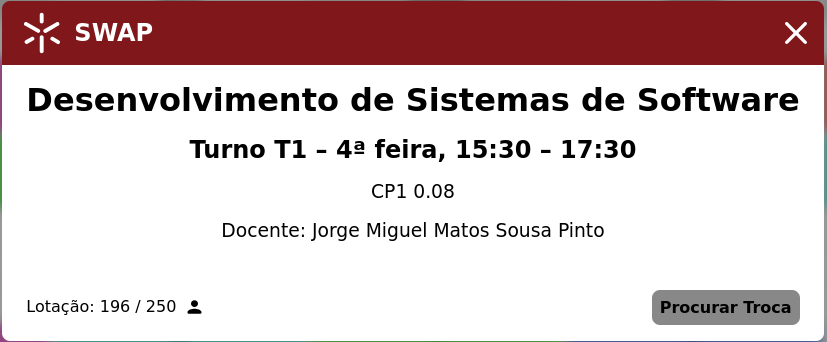
\includegraphics[height=4cm]{res/components/popup-1.png}
    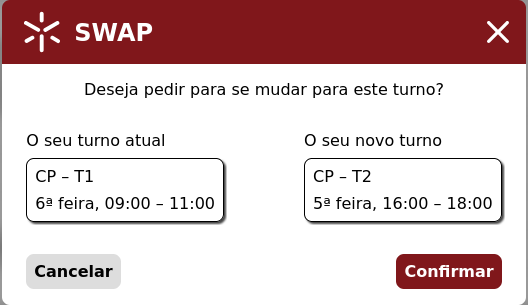
\includegraphics[height=4cm]{res/components/popup-2.png}
    \caption{Diálogos de informação de turno e para confirmação de troca de turnos.}
    \label{popup}
\end{figure}

\subsection{Seletor de turnos}

Este componente, presente nas páginas ``Horário Completo'' e ``Gerir Turnos'', permite ao utilizador
escolher que turnos deseja ver no horário apresentado.

\begin{figure}[H]
    \centering
    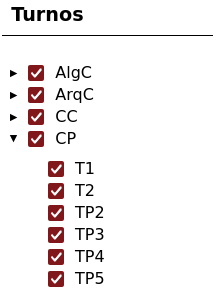
\includegraphics[width=4cm]{res/components/shift-selector.png}
    \caption{Seletor de turnos.}
    \label{shift-selector}
\end{figure}

\subsection{\emph{Toast}}

Este trata-se de um componente para apresentar um alerta ao utilizador, sem que este deixe de poder
utilizar a página. É normalmente utilizado para informar o utilizador de sucesso nas operações que
realizou: que um pedido de mudança de horário foi enviado nas páginas ``O Meu Horário'' e
``Horário Completo'', e que os horários foram publicados com sucesso, na página
``Resolver Problemas''. Abaixo, pode ver-se o exemplo de uma \emph{toast}:

\begin{figure}[H]
    \centering
    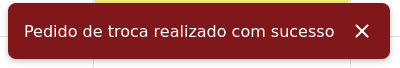
\includegraphics[width=8cm]{res/components/toast.png}
    \caption{\emph{Toast}.}
    \label{toast}
\end{figure}

\subsection{Turno}

Este componente, utilizado no componente ``Horário'' (figura \ref{schedule}), permite apresentar um
turno. Existem várias variantes de turnos, necessárias para ser possível distinguir turnos com os
quais é possível interagir, turnos pertencentes ao horário do aluno, o turno do qual um aluno
requisita para sair, \emph{etc.}. É também possível escolher se se deseja que um turno apresente ou
não a sua capacidade.

\subsection{Botão com ícone}

Este componente trata-se de um \emph{widget} no qual se pode clicar para se realizar uma ação,
sendo utilizado no componente ``Notificação'', do diretor de curso (figura \ref{notification}).
Existem várias variantes para as ações de rejeitar, aprovar ou navegar para a página de resolução
de um pedido, distinguíveis pelo seu ícone. Abaixo podem ser vistos os três tipos do botão
implementados:

\begin{figure}[H]
    \centering
    
\includegraphics[width=4cm]{res/components/icon-button.png}
    \caption{Da esquerda para a direita, variantes de rejeição, aprovação e navegação dos botões.}
    \label{icon-button}
\end{figure}

\subsection{Notificação}

Este componente, utilizado no componente ``Lista de Notificações'' (figura
\ref{notifications-list}), permite apresentar o conteúdo e estado de uma notificação / pedido
(troca de turno, de sala, ou alerta). Existem várias variantes deste componente, apresentadas a
diferentes utilizadores em diferentes cenários (notificação de aluno, do director de curso, ou
pedido). Adicionalmente, notificações do diretor de curso, quando sobrevoadas pelo cursor,
apresentam três botões, que permitem rejeitar, aprovar ou navegar para a página de resolução do
pedido apresentado na notificação. As variantes do diretor de curso e de um pedido podem observar-se
abaixo:

\begin{figure}[H]
    \centering
    
\includegraphics[width=\textwidth]{res/components/director-notification.png}
    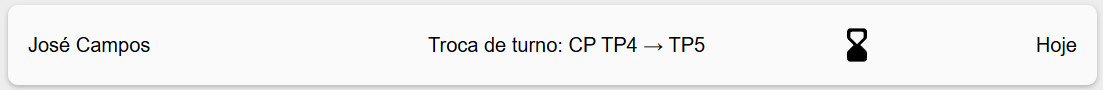
\includegraphics[width=\textwidth]{res/components/student-request.png}
    \caption{De cima para baixo, variantes notificação de diretor de curso e de pedido.}
    \label{notification}
\end{figure}

\subsection{Lista de Notificações}

Este componente, utilizado nas páginas de ``Histórico de Pedidos'' e ``Notificações'', apresenta uma
lista de notificações / pedidos, em que cada elemento é uma instância do componente ``Notificação''.
Permite listar as notificações / pedidos de um utilizador, organizados temporalmente e por estado do
pedido, como se pode ver abaixo:

\begin{figure}[H]
    \centering
    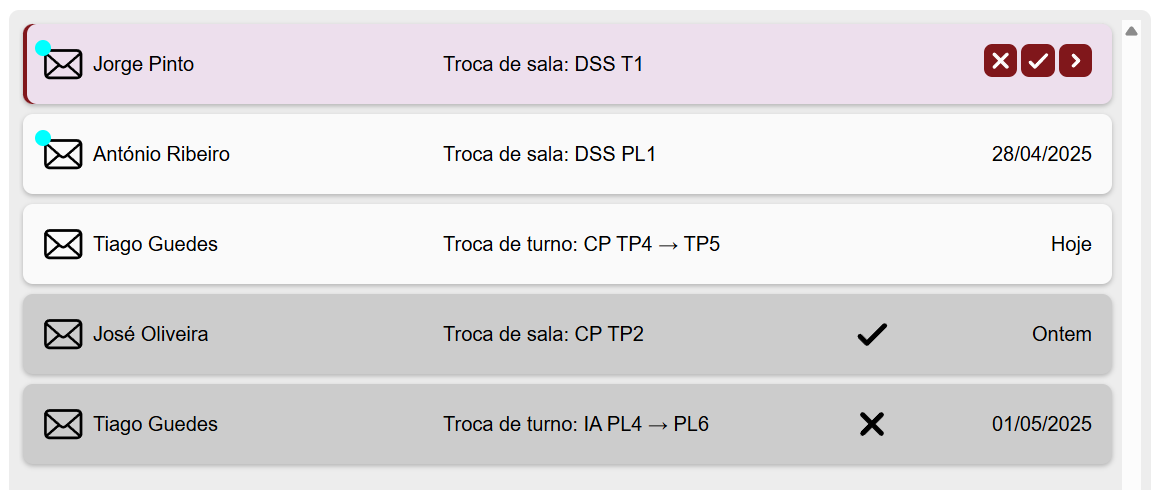
\includegraphics[width=\textwidth]{res/components/director-notifications-list.png}
    \caption{Lista de notificações, do diretor de curso.}
    \label{notifications-list}
\end{figure}

\section{Páginas Implementadas}

Para não repetir o mesmo conteúdo duas vezes neste relatório, as páginas implementadas são
apresentas na secção ``\nameref{user-manual}''.

\section{Tecnologias Utilizadas}

Para a realização deste projeto, foi necessário o uso de diversas tecnologias. Nesta secção,
procura-se apresentar as diversas tecnologias utilizadas, como estas foram utilizadas, e as
facilidades e dificuldades sentidas com cada uma.

\subsection{HTML e CSS}

Visto que a aplicação desenvolvida é uma aplicação Web, o uso de HTML e CSS é imperativo em quase
todas as \emph{frameworks}. De um modo geral, o desenvolvimento de componentes e páginas com recurso
a estas tecnologias foi fácil, especialmente devido à sua natureza declarativa. Outra facilidade do
uso destas tecnologias foram as \emph{flexboxes}, que simplificaram a organização dos elementos nos
componentes e nas páginas.

No entanto, houve algumas dificuldades em garantir que o código desenvolvido funcionava em todos os
navegadores: como nem todos os navegadores suportavam todas as funcionalidades desejadas, foi
necessário testar a aplicação desenvolvida em Chromium (Blink), Firefox (Gecko) e Safari (WebKit).
Várias vezes, foi necessário adicionar regras de CSS com \emph{vendor prefixes}, ou até refazer
algumas funcionalidades devido a diferenças de funcionamento entre navegadores.

\subsection{TypeScript}

\hyphenation{Java-Script}

No projeto desenvolvido, foi utilizado TypeScript \cite{typescript}, linguagem que é transpilada
para JavaScript, mas que permite alguma verificação de tipos. O TypeScript foi uma grande ajuda para
garantir a correção do código da aplicação, e assegurar, em \emph{compile-time}, que a aplicação não
teria exceções em \emph{runtime} devido a erros de tipos. Ademais, o compilador não obriga que o
código seja tipado durante o processo de desenvolvimento, pelo que este pode continuar a ser
bastante veloz. Assim, apenas quando se acaba de escrever um módulo / componente / página, podem
adicionar-se anotações de tipo ao código para garantir a sua correção.

\subsection{Vue}

A \emph{framework} utilizada para o desenvolvimento da aplicação foi Vue.js \cite{vue}. Esta
\emph{framework}, devido à sua natureza declarativa e reativa, foi de muito fácil atualização:
alterar um objeto reativo conduzia à atualização automática das partes do componente / da página que
sofreram alterações. Por exemplo, ao contrário do Blazor \cite{blazor}, utilizado em Laboratórios de
Informática IV, não era necessário chamar uma função (\texttt{StateHasChanged}) sempre que era
necessário atualizar os conteúdos da DOM.

Apesar de poucas, foram sentidas algumas dificuldades no uso de Vue, especialmente quando era
necessário integrar funcionalidades não reativas (no caso, a resposta a um evento de mudança de uma
\emph{media query}) com a reatividade do Vue, tendo sido necessários \emph{hacks} para forçar a
atualização dos objetos reativos.

\subsection{Pinia}

A biblioteca Pinia \cite{pinia} foi utilizada para armazenamento do estado da aplicação, como as
credenciais do utilizador, o tema da aplicação (claro ou escuro) e os turnos escolhidos nas páginas
``Horário Completo'' e ``Gerir Turnos'', para que esta informação não desapareça quando se navega
entre diferentes páginas da aplicação. Adicionalmente, o \emph{plugin}
\texttt{pinia-plugin- persistedstate} \cite{pinia-persistent} foi utilizado para persistir algum
estado no \texttt{localStorage} do navegador, para este ser mantido mesmo após o navegador ser
fechado. Por exemplo, as credenciais do utilizador são armazenadas no \texttt{localStorage} quando
este escolhe que deseja que a aplicação se ``lembre de si''.

O Pinia, devido à sua integração com Vue, foi das ferramentas de mais fácil utilização, visto que os
objetos armazenados nos \emph{stores} do Pinia podiam ser utilizados como qualquer outro objeto
reativo do Vue.

\subsection{JSON Server}

É necessário que a aplicação desenvolvida tenha dados que possa apresentar. Na UC de Interface
Pessoa-Máquina, não é pedido que se implemente um \emph{backend} completo para a aplicação, pelo que
se utilizou \texttt{json-server} \cite{json-server}, um programa que cria uma API REST a partir dos
dados num ficheiro JSON.

A utilização desta tecnologia foi complicada, não devido a complexidade da tecnologia em si, mas sim
devido ao trabalho necessário para organizar os dados da API num formato adequado para apresentação.
Devido às capacidades muito limitadas de interrogação do \texttt{json-server}, várias interrogações
tiveram de ser implementadas imperativamente em JavaScript, ao contrário de declarativamente numa
linguagem especializada, como se teria feito caso se tivesse utilizado uma base de dados. O uso de
uma base de dados seria, por este motivo, uma grande melhoria ao projeto.

\subsection{Outras tecnologias}

O \texttt{npm} \cite{npm} é o gestor de pacotes do NodeJS, que permite, no ficheiro
\texttt{pacakage.json}, definir as dependências do projeto desenvolvido. Além disso, também é
possível definir \emph{scripts} como \texttt{npm run dev}, para abrir a aplicação com ferramentas de
desenvolvimento, e \texttt{npm run preview}, para pré-visualização da aplicação final. Para melhorar
a experiência de desenvolvimento, estes dois \emph{scripts} foram modificados para, além de
executarem o servidor HTTP da aplicação, também executarem o JSON Server. Também foram adicionados
\emph{scripts} para, com recurso às ferramentas ESLint \cite{eslint} e Prettier \cite{prettier},
automaticamente fazer uma análise estática e formatação do código, respetivamente. Estes
\emph{scripts} são usados na \emph{pipeline} de CI (\emph{Continuous Integration}) do repositório do
projeto (GitHub Actions), obrigando a que todos os \emph{pull requests} tenham código correto e bem
formatado.

A principal dificuldade do uso do \texttt{npm} foi garantir que os \emph{scripts} criados
funcionavam em diferentes sistemas operativos, visto que alguns comandos utilizados apenas estavam
disponíveis, por exemplo, em Linux.

\section{Manual de Utilização}
\label{user-manual}

\subsection{Diretor de Curso}

\subsubsection{Cenário 1}

Neste cenário, o diretor de curso entra na aplicação, consulta a ocupação dos turnos, e aloca os
alunos que o algoritmo de geração de horários automático não alocou. Finalmente, publica o horário
dos alunos. Para isso, terá de realizar os seguintes passos:

\textbf{- Iniciar sessão com as suas credenciais:}

Preencher o ecrã seguinte com o seu endereço eletrónico e palavra-passe, terminando a clicar no
botão ``Iniciar Sessão'':

\begin{figure}[H]
    \centering
    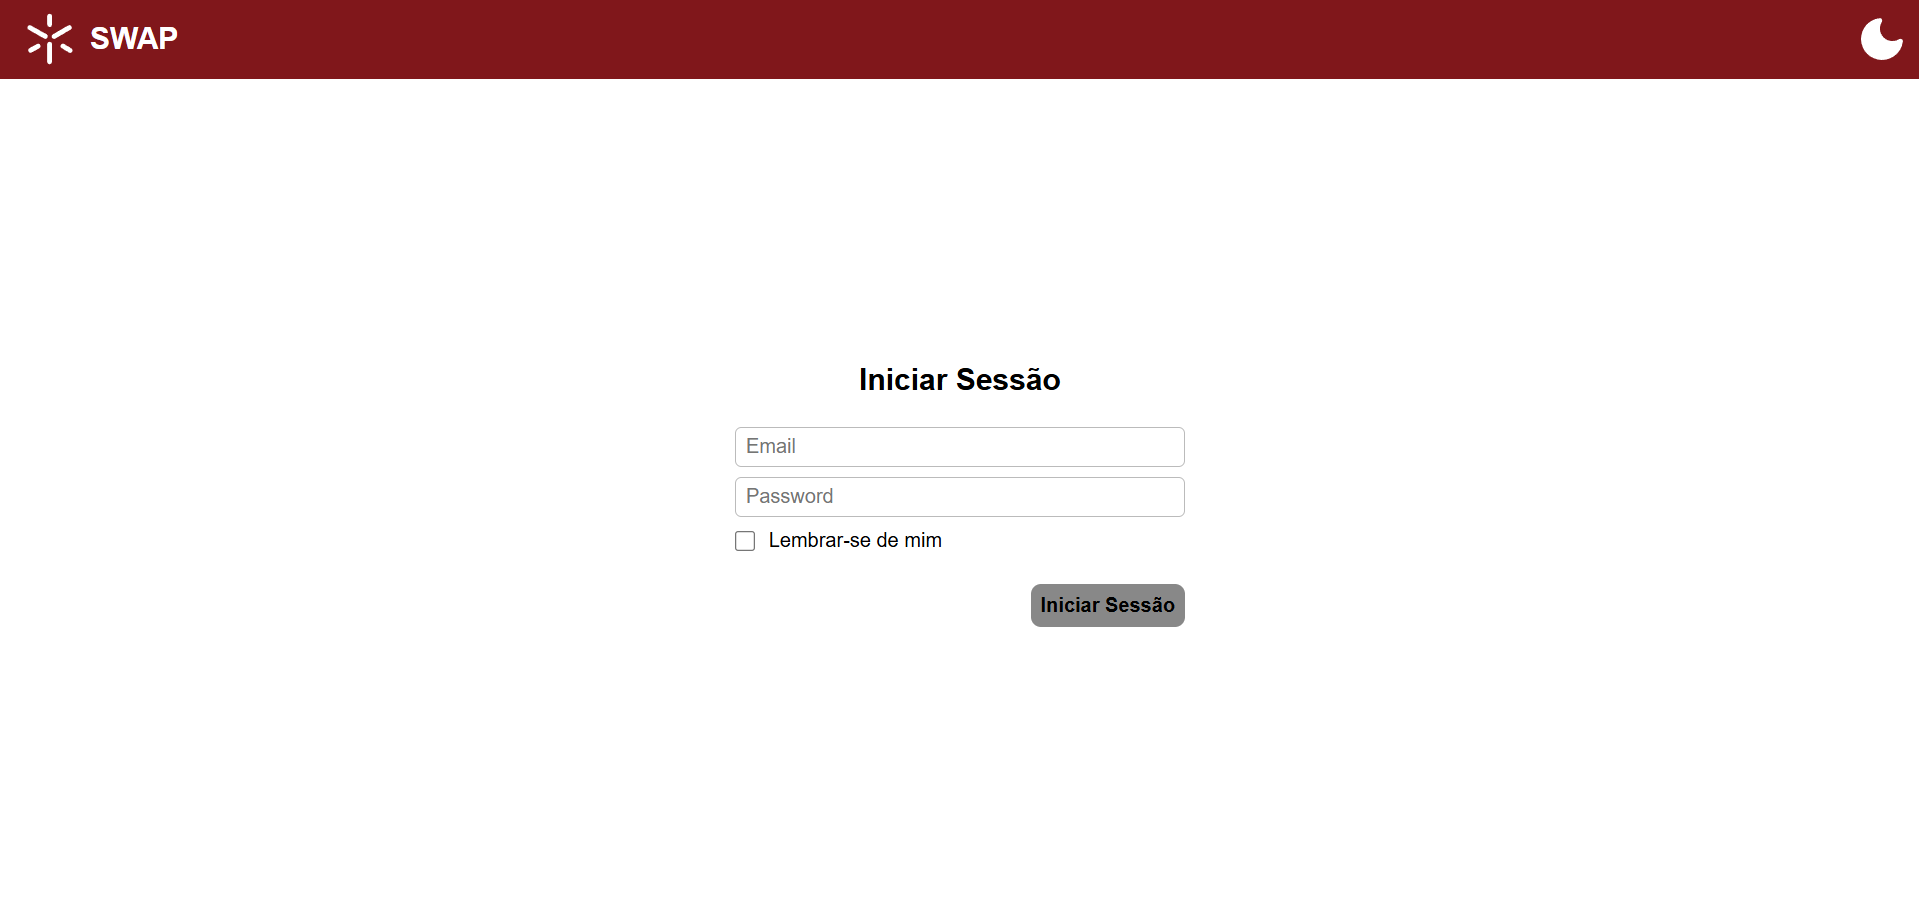
\includegraphics[width=0.8\textwidth]{res/manual/pagina_login_vazia.png}
    \caption{Página ``Iniciar Sessão'' por preencher.}
    \label{pagina_login_vazia}
\end{figure}

\begin{figure}[H]
    \centering
    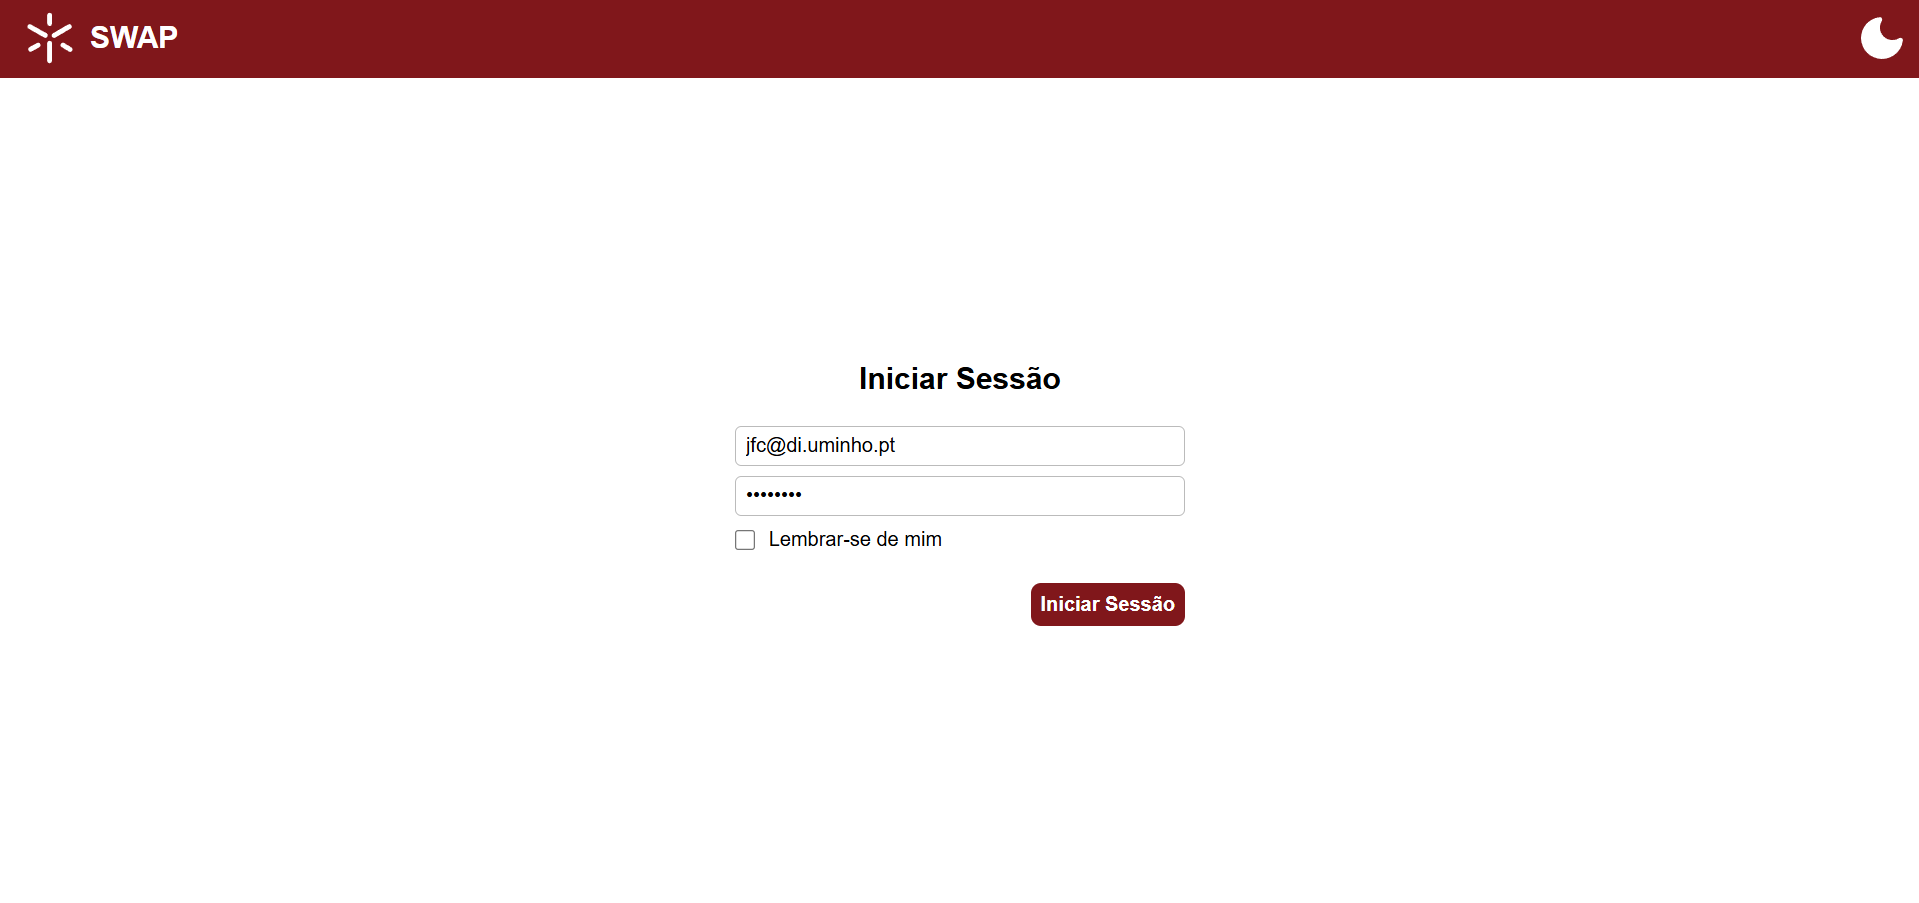
\includegraphics[width=0.8\textwidth]{res/manual/login_diretor.png}
    \caption{Página``Iniciar Sessão'' preenchida com credenciais.}
    \label{login_diretor}
\end{figure}

\textbf{- Ver a ocupação dos turnos:}

A aplicação desenvolvida procura minimizar o esforço de memória necessário para a sua utilização.
Não é necessário que o diretor de curso consulte a capacidade dos turnos para saber onde pode e não
pode colocar alunos (ver página ``Resolver Problemas'' abaixo). Mesmo assim, pode fazê-lo, como se
mostra nesta secção, primeiro acedendo à página ``Gerir Turnos'':

\begin{figure}[H]
    \centering
    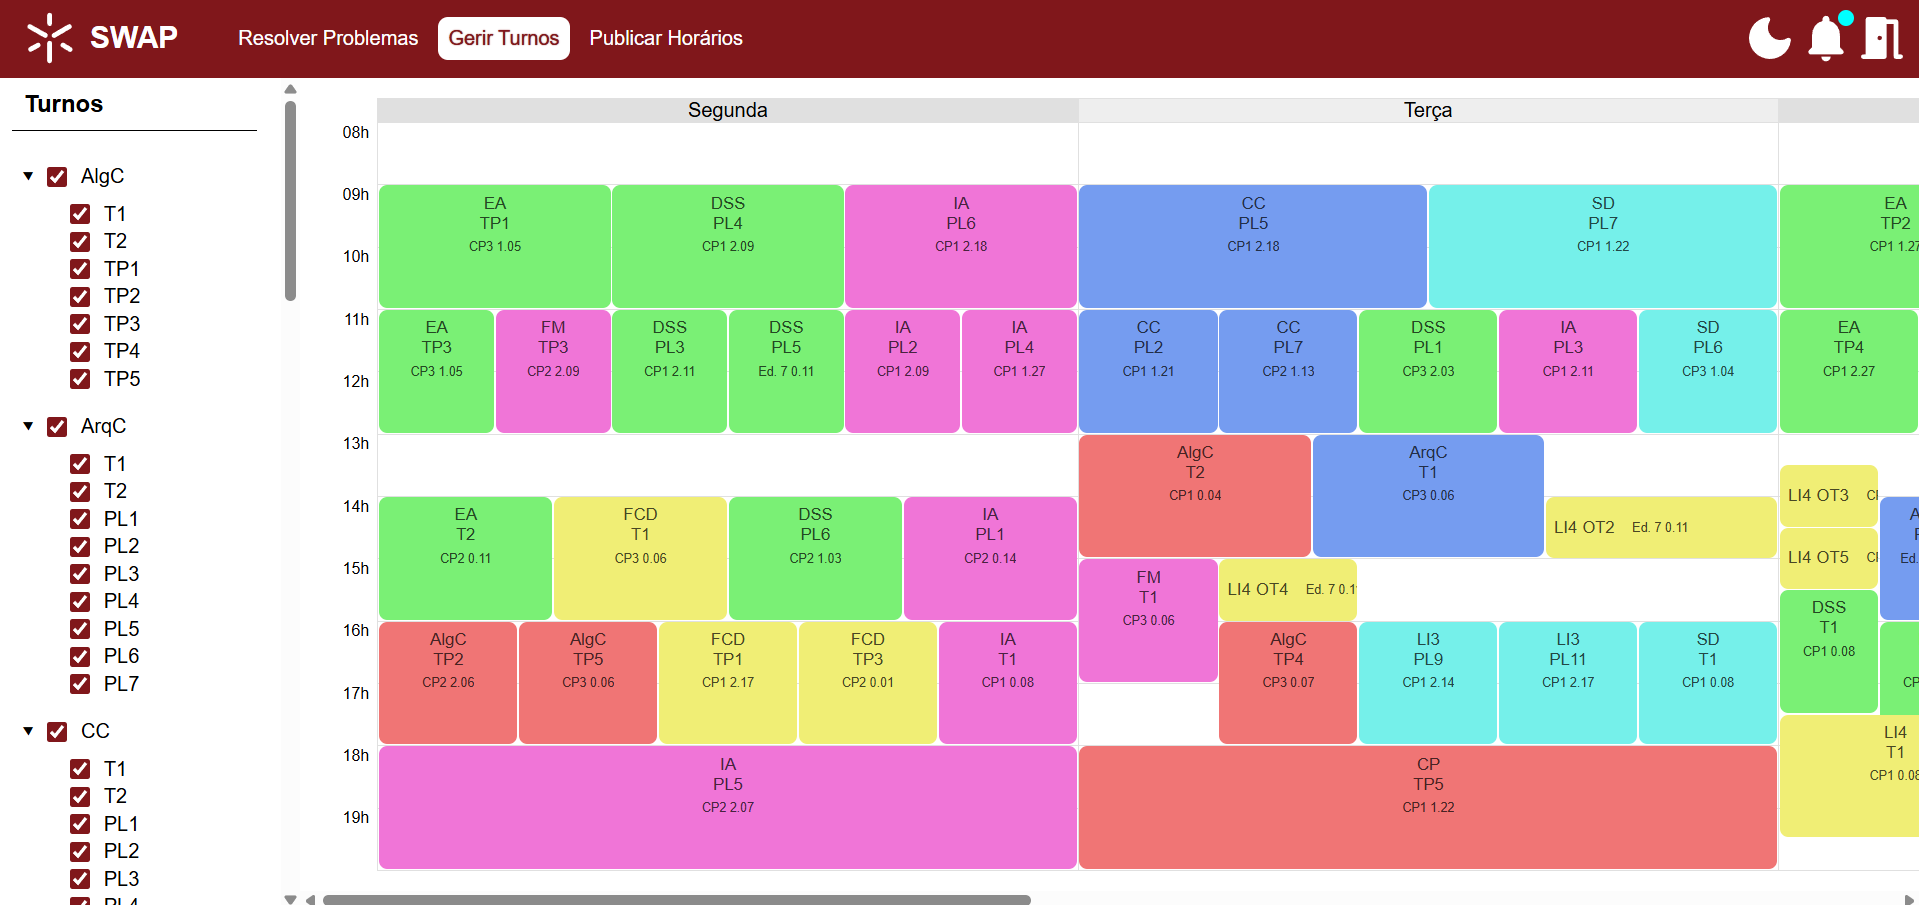
\includegraphics[width=0.8\textwidth]{res/manual/gerir_turnos.png}
    \caption{Página ``Gerir Turnos''.}
    \label{gerir_turnos}
\end{figure}

É possível, através da barra lateral, selecionar que turnos são apresentados no horário, caso alguns
turnos ou UCs não sejam de grande interesse para a tarefa atual do diretor de curso:

\begin{figure}[H]
    \centering
    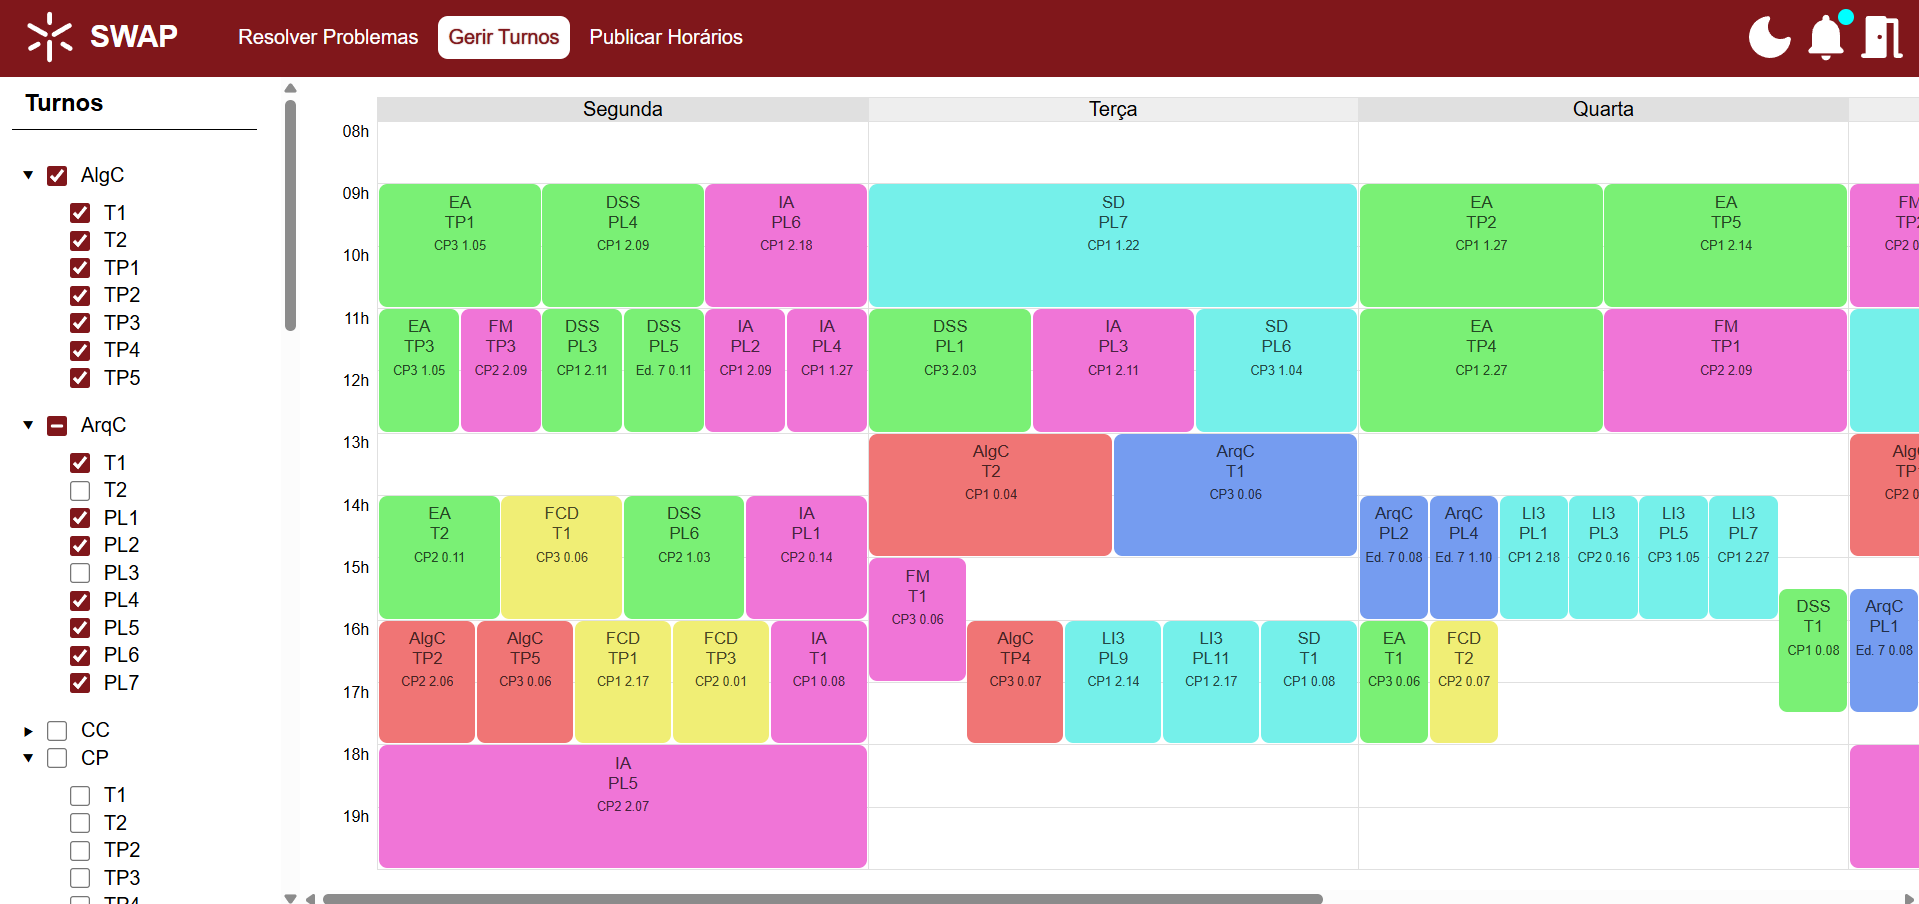
\includegraphics[width=0.8\textwidth]{res/manual/gerir_turnos_filtrados.png}
    \caption{Página ``Gerir Turnos'' com alguns turnos por selecionar.}
    \label{gerir_turnos_filtrados}
\end{figure}

Clicando num turno, o utilizador será redirecionado para a página ``Gerir Turno'', onde, para além
de outras funcionalidades descritas posteriormente, pode consultar a sua lotação:

\begin{figure}[H]
    \centering
    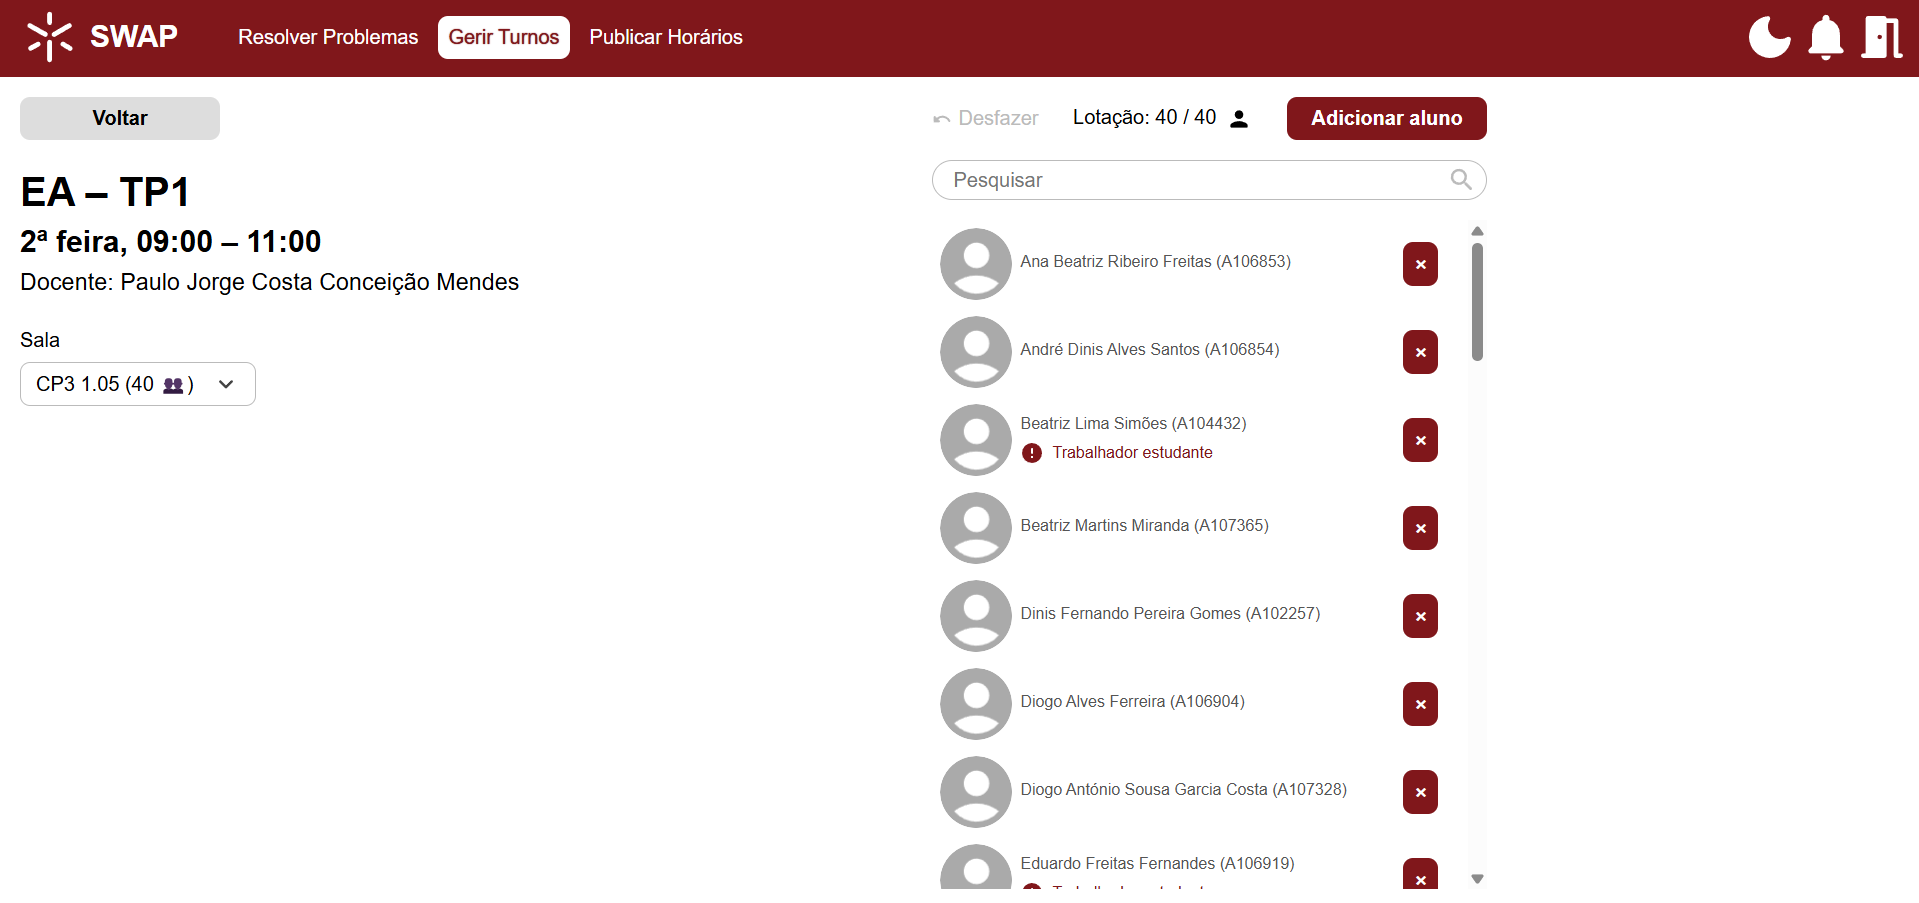
\includegraphics[width=0.8\textwidth]{res/manual/gerir_turno.png}
    \caption{Página ``Gerir Turno''.}
    \label{gerir_turno}
\end{figure}

\textbf{- Consultar alunos não colocados:}

Ao entrar na aplicação, a página ``Resolver Problemas'' é apresentada ao diretor de curso, e mostra
os alunos que não estão colocados num turno e os pedidos de troca de turno. Note-se que esta página
também é acessível a partir da barra de navegação. A lista de problemas é pesquisável, tornando mais
fácil encontrar um problema específico em listas de grande dimensão.

\begin{figure}[H]
    \centering
    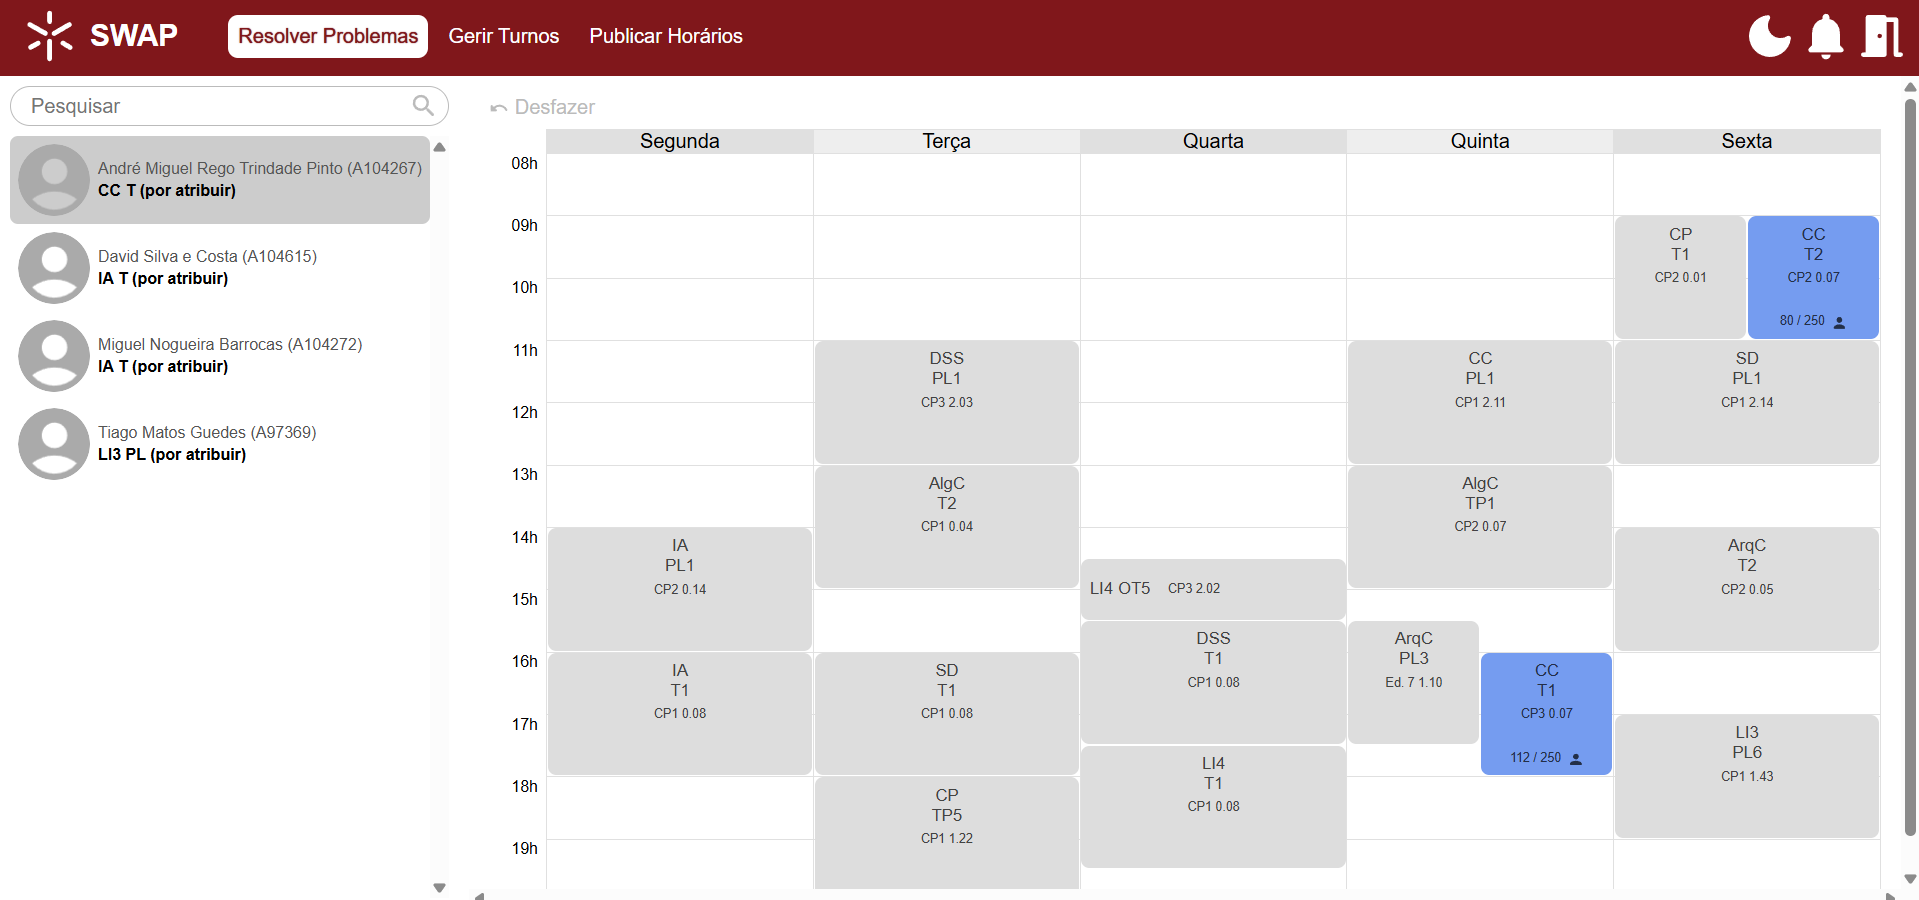
\includegraphics[width=0.8\textwidth]{res/manual/resolver_problemas.png}
    \caption{Página ``Resolver Problemas''.}
    \label{resolver_problemas}
\end{figure}

\begin{figure}[H]
    \centering
    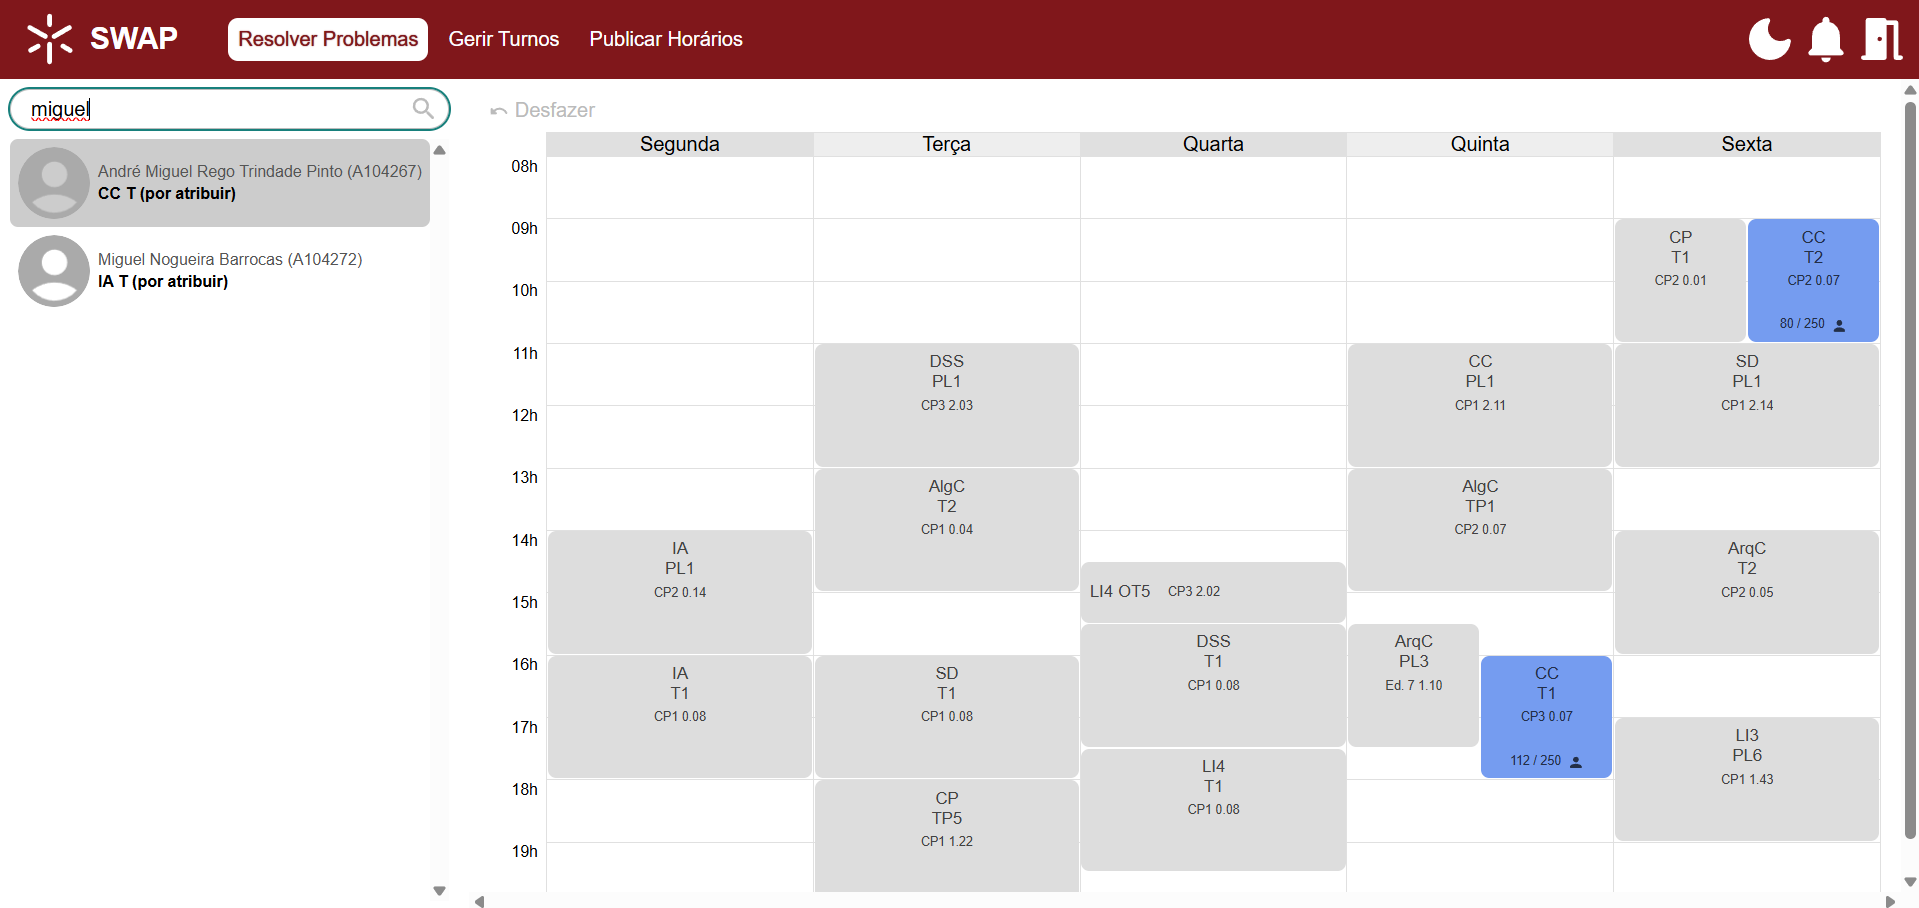
\includegraphics[width=0.8\textwidth]{res/manual/resolver_problemas_pesquisar.png}
    \caption{Página ``Resolver Problemas'' durante uma pesquisa por um aluno.}
    \label{resolver_problemas_pesquisa}
\end{figure}

\textbf{- Alocação manual:}

O diretor de curso pode, nesta página, clicar num aluno da lista para o tentar alocar a um turno.
Pode ver o horário desse aluno e os turnos selecionáveis, bem como a lotação dos mesmos, para assim
tentar escolher um turno com vagas disponíveis que não crie conflitos no horário. Para colocar o
aluno nesse turno de forma provisória, basta clicar no turno pretendido.

\textbf{- Publicar horário:}

Para fazer com que as mudanças efetuadas fiquem guardadas e afetem o horário dos alunos, o diretor
de curso deve aceder à página ``Publicar Horários'' e clicar no botão com o mesmo nome. Esta página
apresenta sempre os problemas por revolver, lembrando ao diretor de curso de que pode estar a
cometer um erro caso esteja a publicar horários ainda com turnos por atribuir e pedidos por
satisfazer.

\begin{figure}[H]
    \centering
    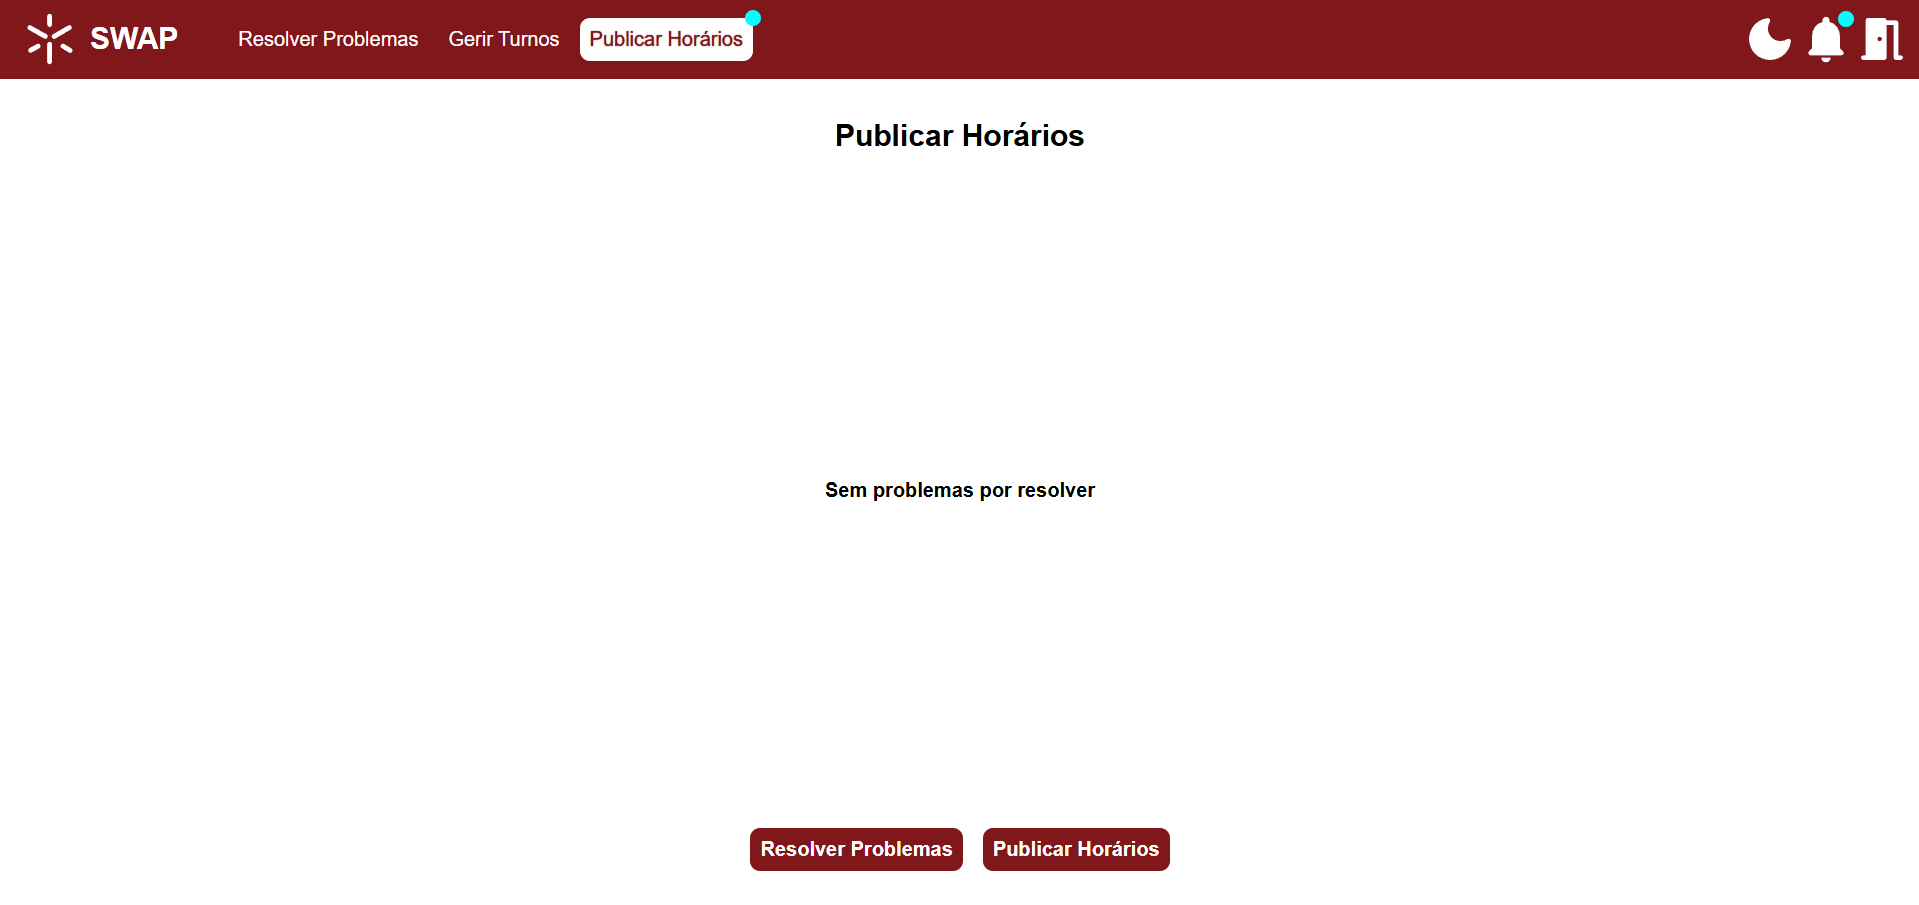
\includegraphics[width=0.8\textwidth]{res/manual/publicar_horario.png}
    \caption{Página ``Publicar Horários''.}
    \label{publicar_horarios}
\end{figure}

Após publicar os horários, o utilizador será redirecionado para a página ``Resolver Problemas'', e
surgirá uma confirmação de que os horários foram publicados:

\begin{figure}[H]
    \centering
    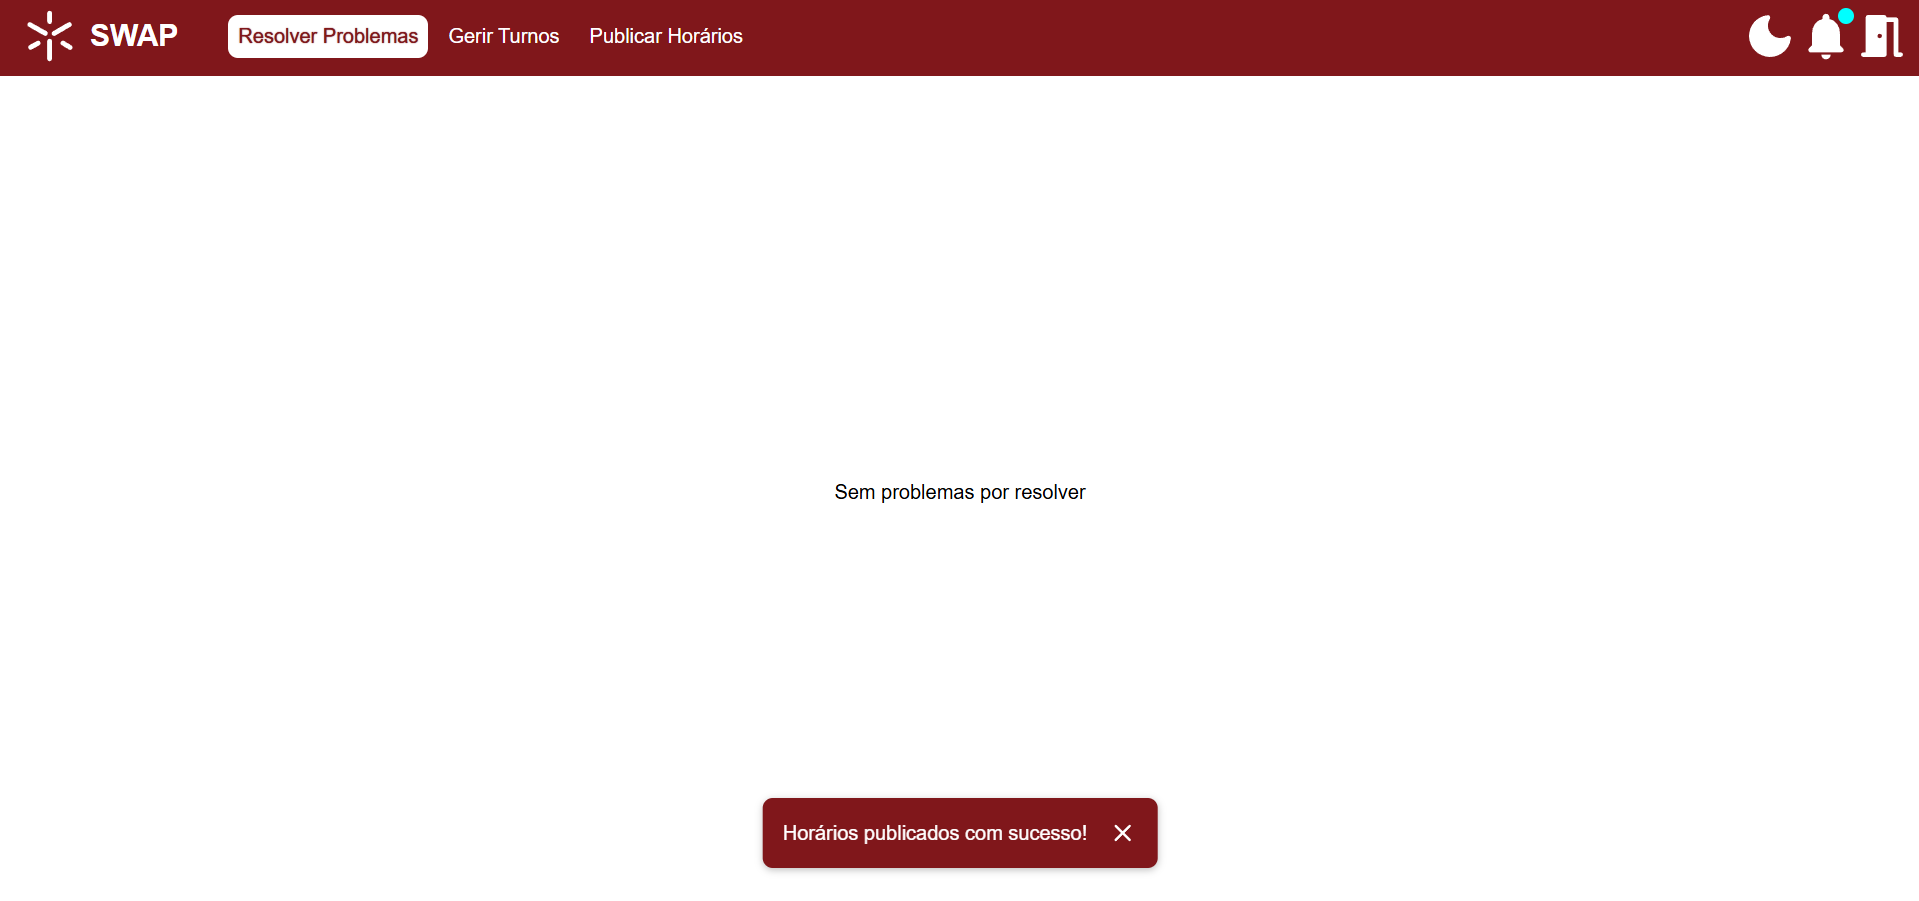
\includegraphics[width=0.8\textwidth]{res/manual/toast_horario_publicado.png}
    \caption{Confirmação da publicação de horários.}
    \label{toast_horario_publicado}
\end{figure}

\subsubsection{Cenário 2}

Para as operações descritas no cenário 2, em que o diretor de curso responde a um pedido de mudança
de sala, ele terá de realizar as seguintes ações:

\textbf{- Ver os pedidos:}

Para ver os pedidos feitos pelos docentes, o diretor de curso irá consultar as suas notificações,
clicando no botão com ícone de sino, no canto superior direito da página. Sobrevoando o cursor ao
pedido, terá três opções: rejeitá-lo, aceitá-lo ou visualizá-lo:

\begin{figure}[H]
    \centering
    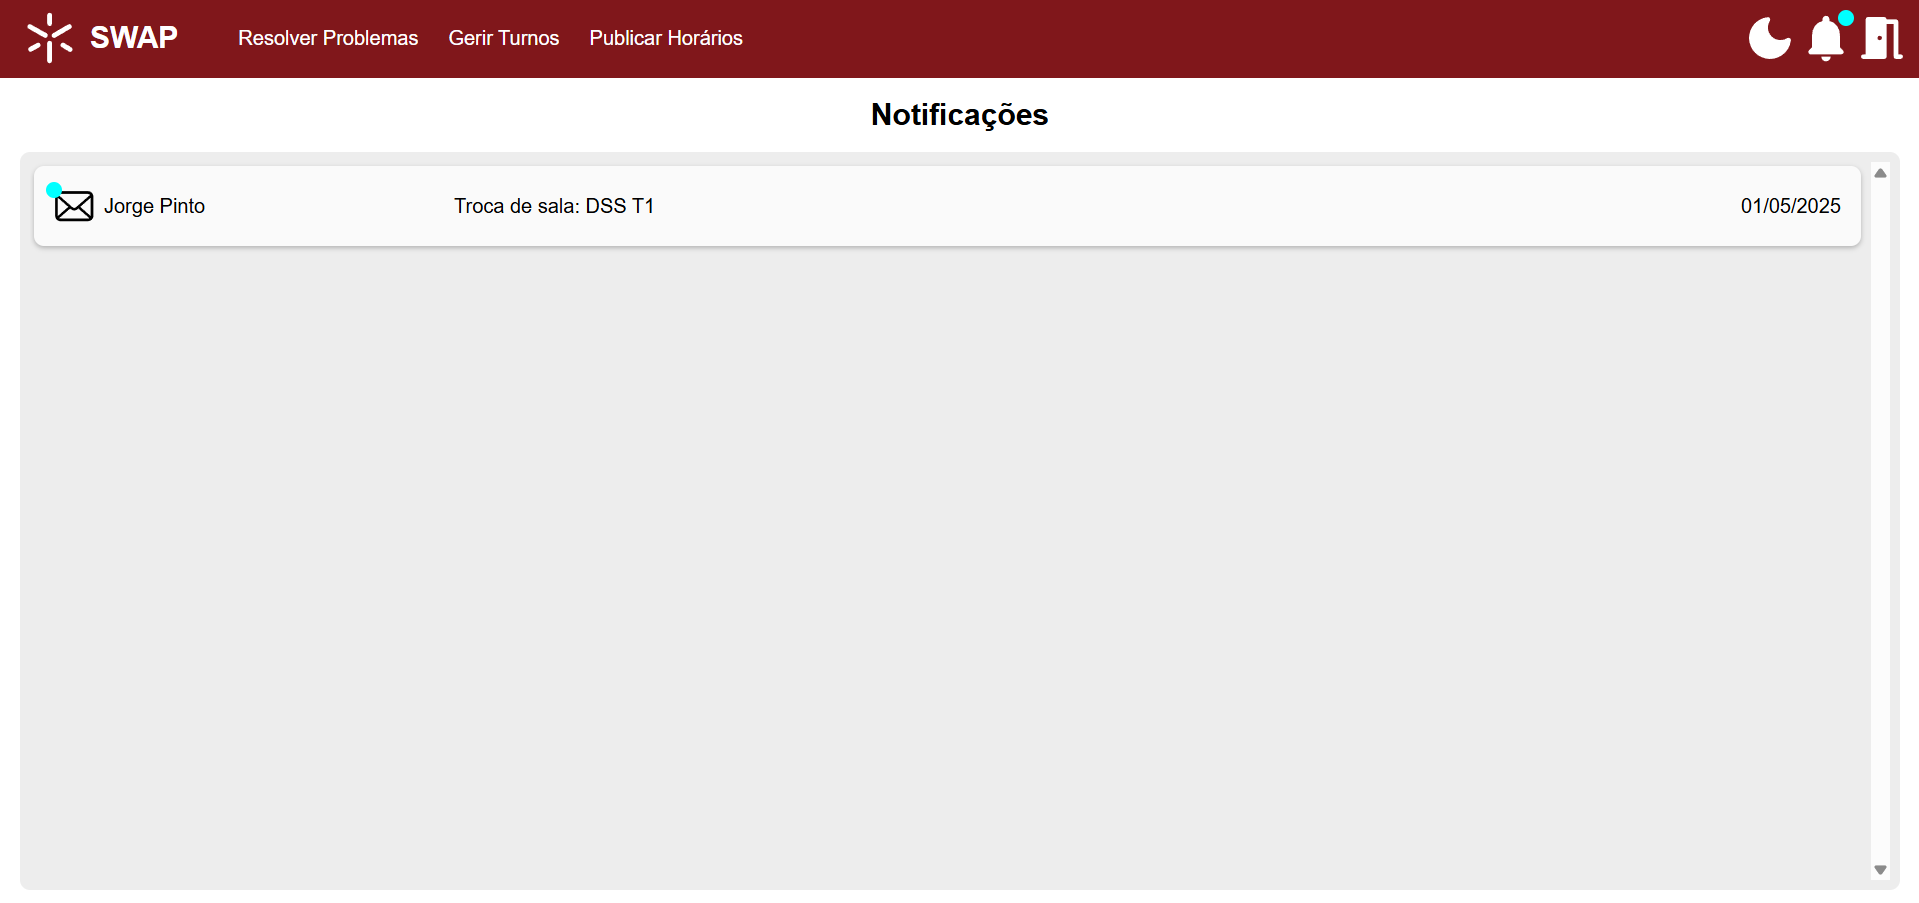
\includegraphics[width=0.8\textwidth]{res/manual/notificacao_troca_sala.png}
    \caption{Notificação de troca de sala na página ``Notificações do Diretor de Curso''.}
    \label{notificacao_troca_sala}
\end{figure}

\begin{figure}[H]
    \centering
    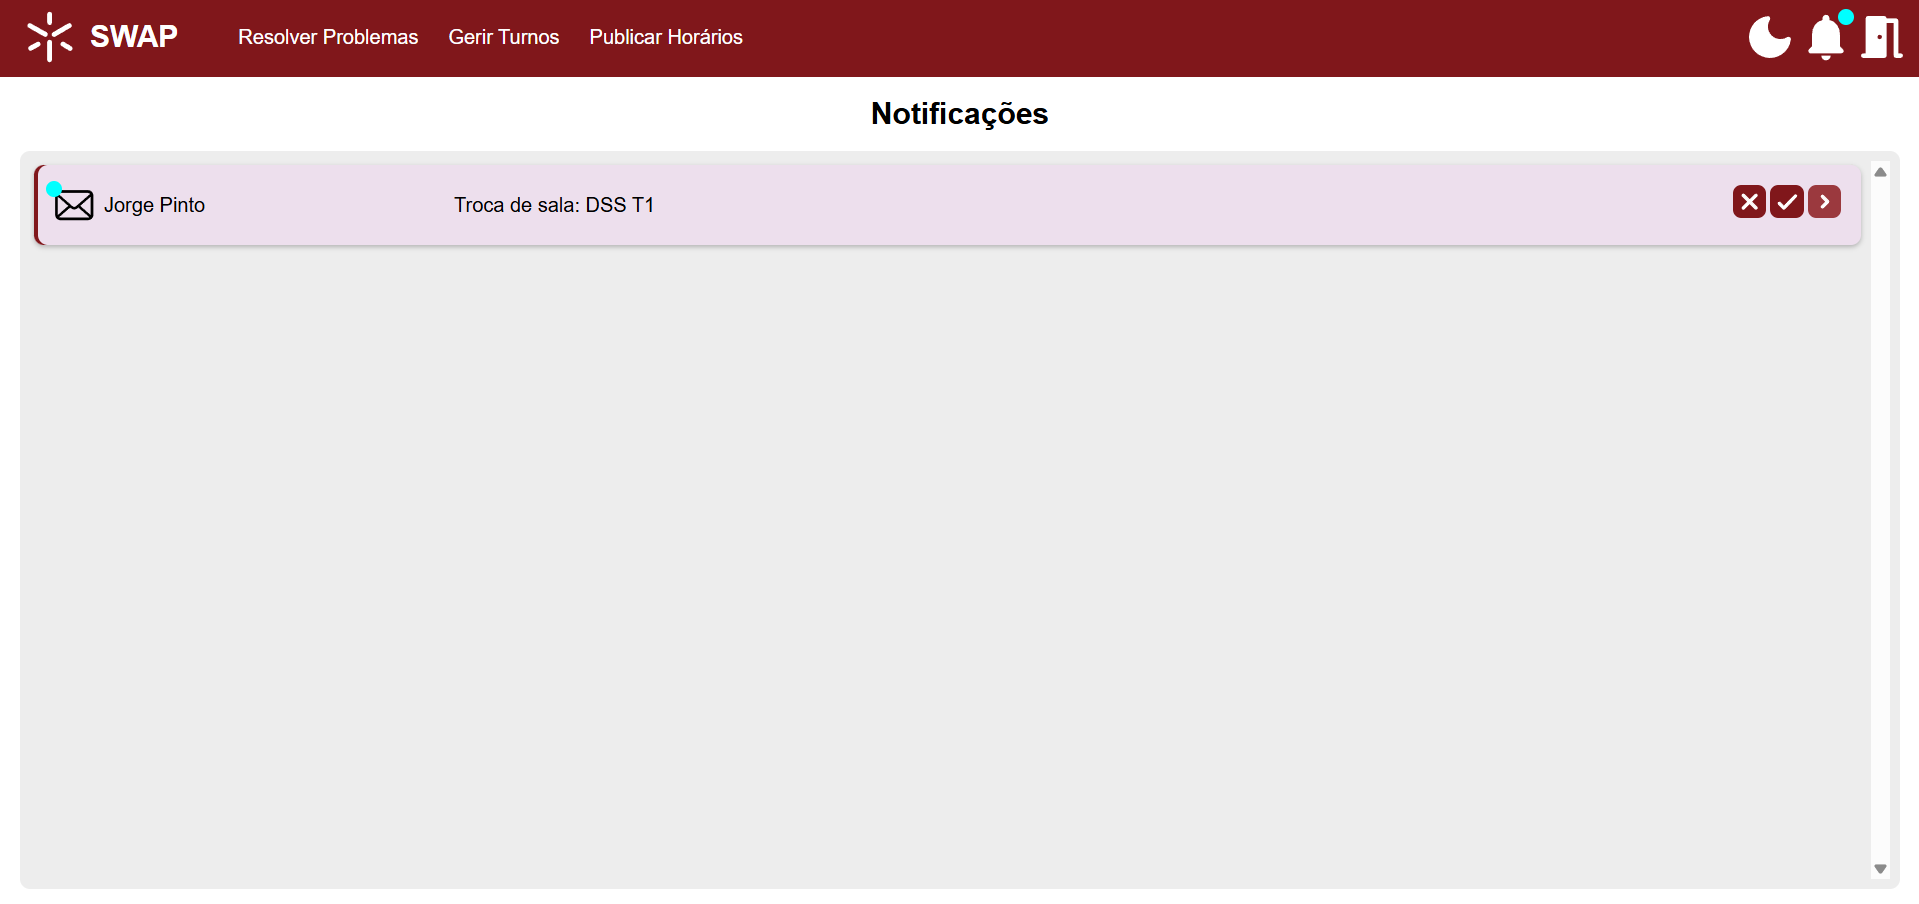
\includegraphics[width=0.8\textwidth]{res/manual/notificacao_troca_sala_hover.png}
    \caption{Opções de uma notificação na página ``Notificações do Diretor de Curso''.}
    \label{notificacao_troca_sala_hover}
\end{figure}

As opções de rejeitar e aceitar dão o pedido como resolvido, mostrando ao seu remetente se ele foi
aceite ou rejeitado. A opção de visualizar o pedido leva o utilizador para a página onde este pode
ser resolvido. Neste caso, o diretor, clicando nessa última opção, é redirecionado para a página
``Gerir Turno'' (figura \ref{gerir_turno}).

\textbf{- Consultar as salas disponíveis:}

Nesta página, clicando no \emph{dropdown} ``Sala'', o diretor pode ver as salas disponíveis no
horário daquele turno e a capacidade de cada sala. Neste exemplo, pode ver-se que a sala CP2 0.05
tem uma maior capacidade do que a sala atual, pelo que o diretor pode escolher mudar o turno para
essa sala, selecionando-a no \emph{dropdown}.

\begin{figure}[H]
    \centering
    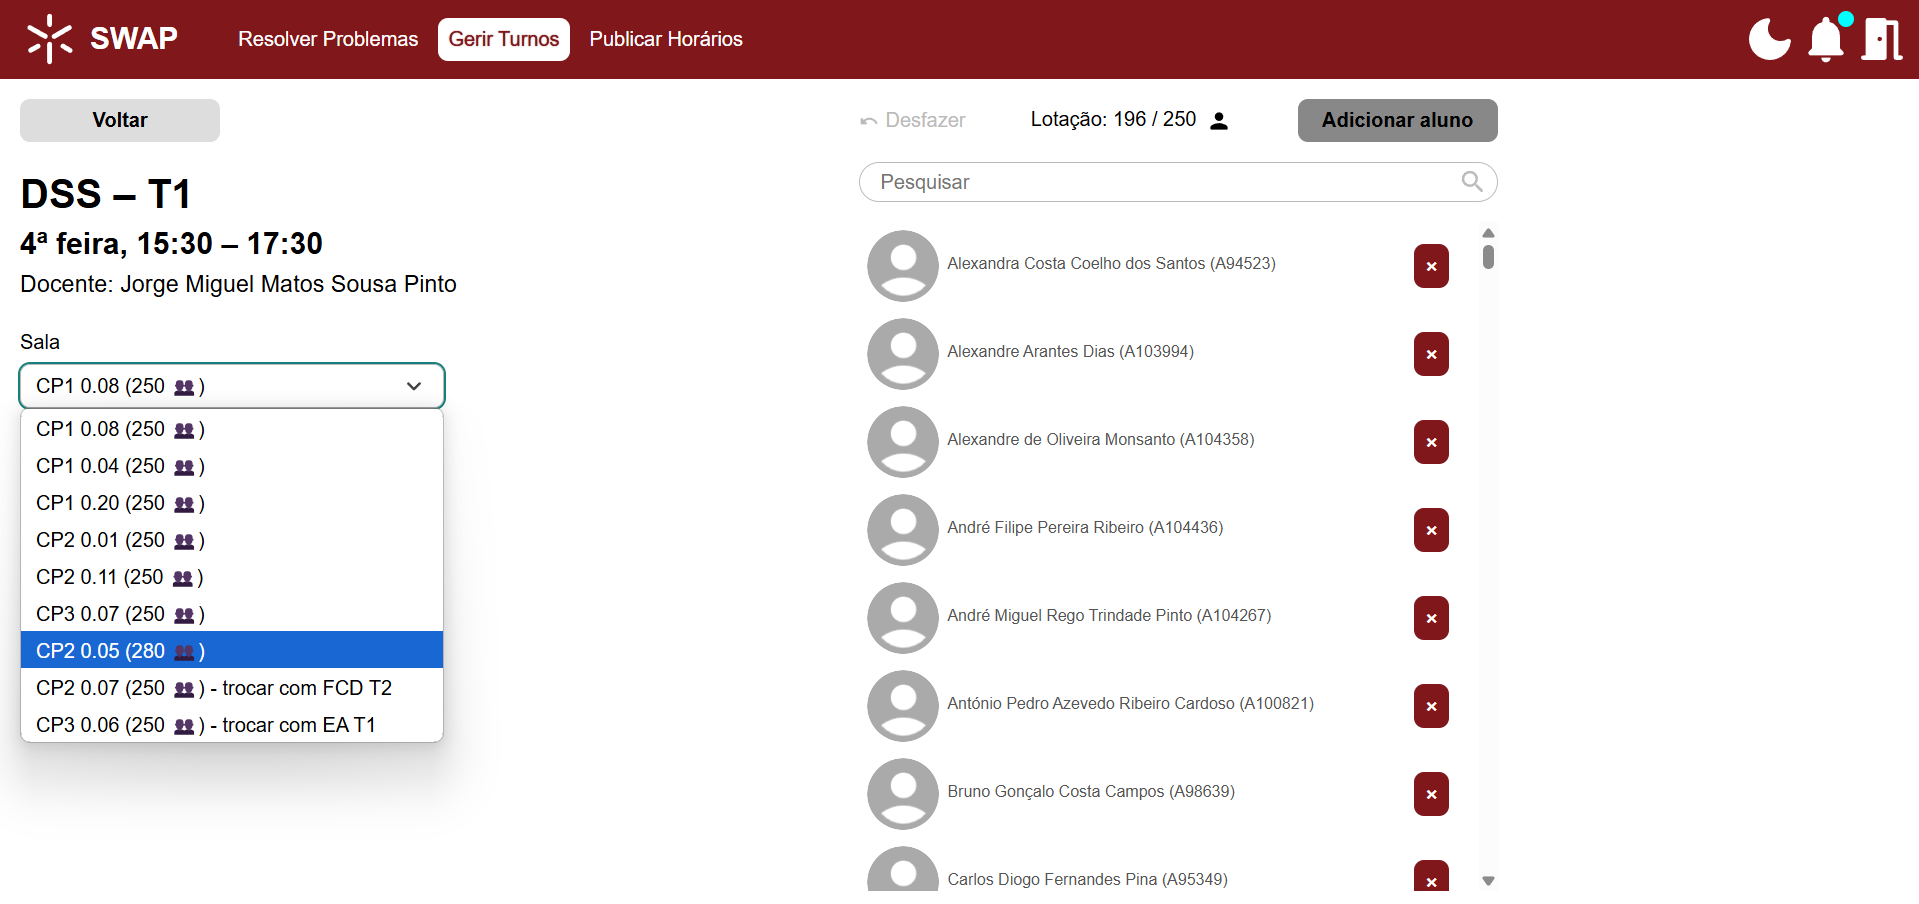
\includegraphics[width=0.8\textwidth]{res/manual/trocar_sala.png}
    \caption{Seleção da sala de um turno na página ``Gerir Turno''.}
    \label{trocar_sala}
\end{figure}

\textbf{- Fazer a alteração da sala:}

Para efetivar a alteração da sala no horário dos alunos, tal como no cenário 1,
o diretor deve publicar o novo horário (figura \ref{publicar_horarios}).

\subsubsection{Cenário 3}

Neste cenário, o diretor de curso vê que existe um pedido de troca de turno, e tenta atender a esse
pedido. Para o fazer, realiza as seguintes ações na aplicação:

\textbf{- Verificar que recebeu um pedido:}

Como mencionado anteriormente, ao entrar na aplicação, a página ``Resolver Problemas'' é apresentada
ao diretor de curso. É nesta página que se encontram também os pedidos efetuados pelos alunos.

\begin{figure}[H]
    \centering
    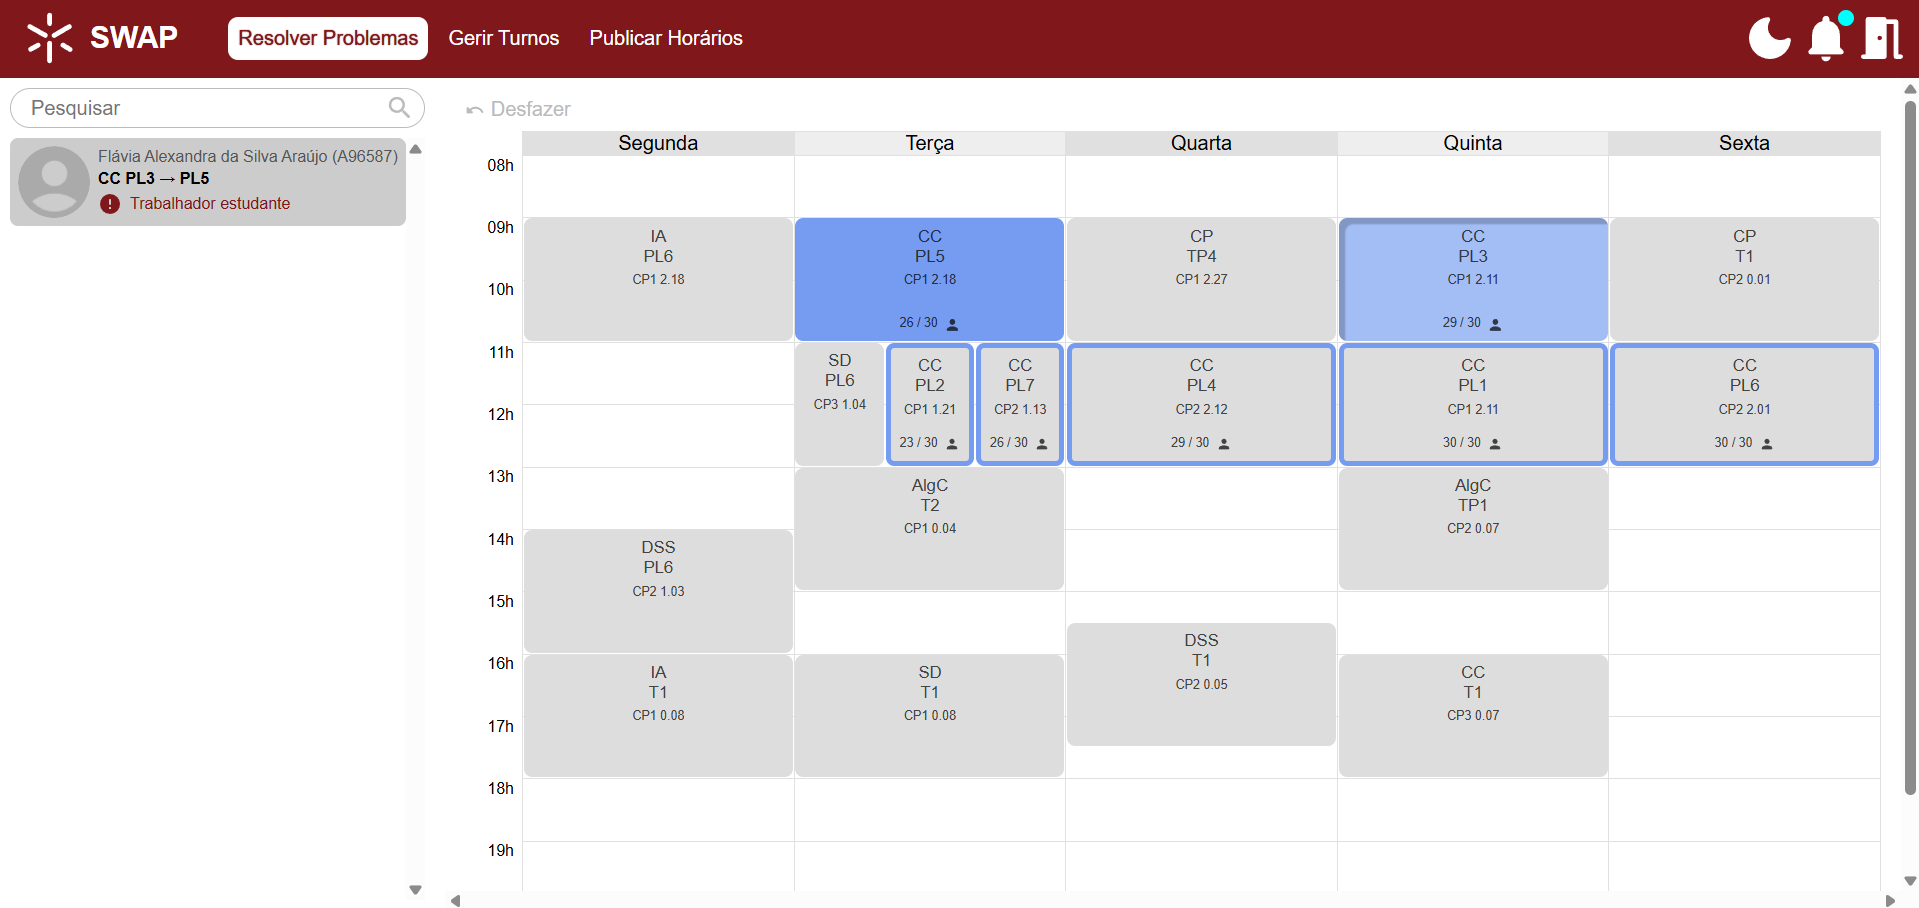
\includegraphics[width=0.8\textwidth]{res/manual/resolver_troca_turno.png}
    \caption{Página ``Resolver Problemas'' com um pedido de troca de turno.}
    \label{resolver_troca_turno}
\end{figure}

O pedido pode também ser visto na página ``Notificações do Diretor de Curso''. Neste caso, o botão
para visualizar um destes pedidos redireciona o utilizador para a página ``Resolver Problemas'', e
não ``Gerir Turnos''.

\begin{figure}[H]
    \centering
    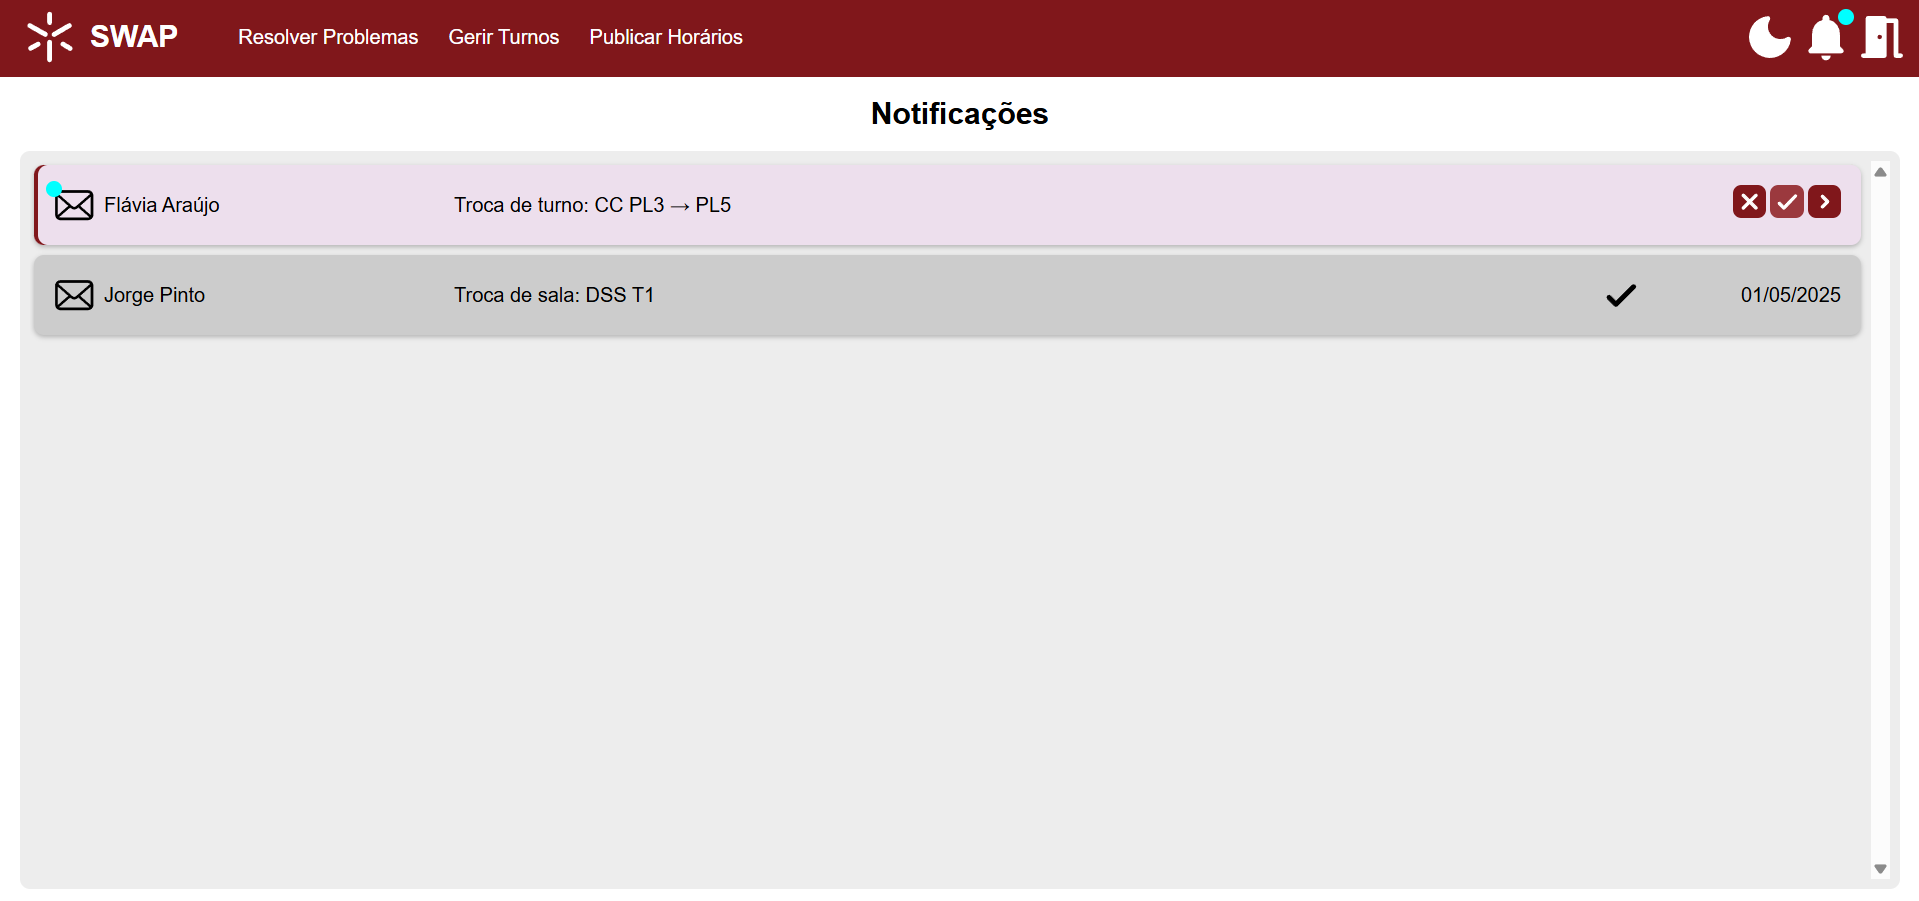
\includegraphics[width=0.8\textwidth]{res/manual/notificacao_troca_turno.png}
    \caption{Página ``Notificações do Diretor de Curso'' com um pedido de troca de turno.}
    \label{notificacao_troca_turno}
\end{figure}

Nesta página, o diretor pode dar o pedido como aceite, sinalizando ao aluno que o pretende resolver,
ou como rejeitado, sinalizando o contrário. Rejeitar um pedido também faz com que o mesmo não
seja apresentado na página ``Resolver Problemas'' (figura \ref{resolver_troca_turno}).

\textbf{- Verificar a capacidade do turno:}

Na página ``Resolver Problemas'' (figura \ref{resolver_troca_turno}), é possível ver, no horário do
aluno que efetuou o pedido, o turno para onde este se pretende mudar, os outros turnos da Unidade
Curricular, e a capacidade de cada um. Assim, pode verificar-se que o turno pretendido pelo aluno, o
PL5, tem vagas disponíveis. No caso de não existir capacidade nesse turno, seria também visível se
outros turnos à mesma hora têm capacidade e, no caso de não existam turnos a essa hora com vagas
disponíveis, é também fácil de ver, pelo aviso na lista de pedidos, que o aluno em questão é
trabalhador estudante, e que se pode abrir uma exceção e violar as restrições de capacidade dos
turnos. Se for esse o caso, ao tentar alocar o aluno, irá aparecer uma mensagem de aviso, que
informa que o turno pretendido está cheio, dando as opções de cancelar a operação, mudar a sala
do turno (desativada no caso dos turnos práticos, porque o que limita a sua capacidade não é a
sala), ou atribuir o turno mesmo assim.

\begin{figure}[H]
    \centering
    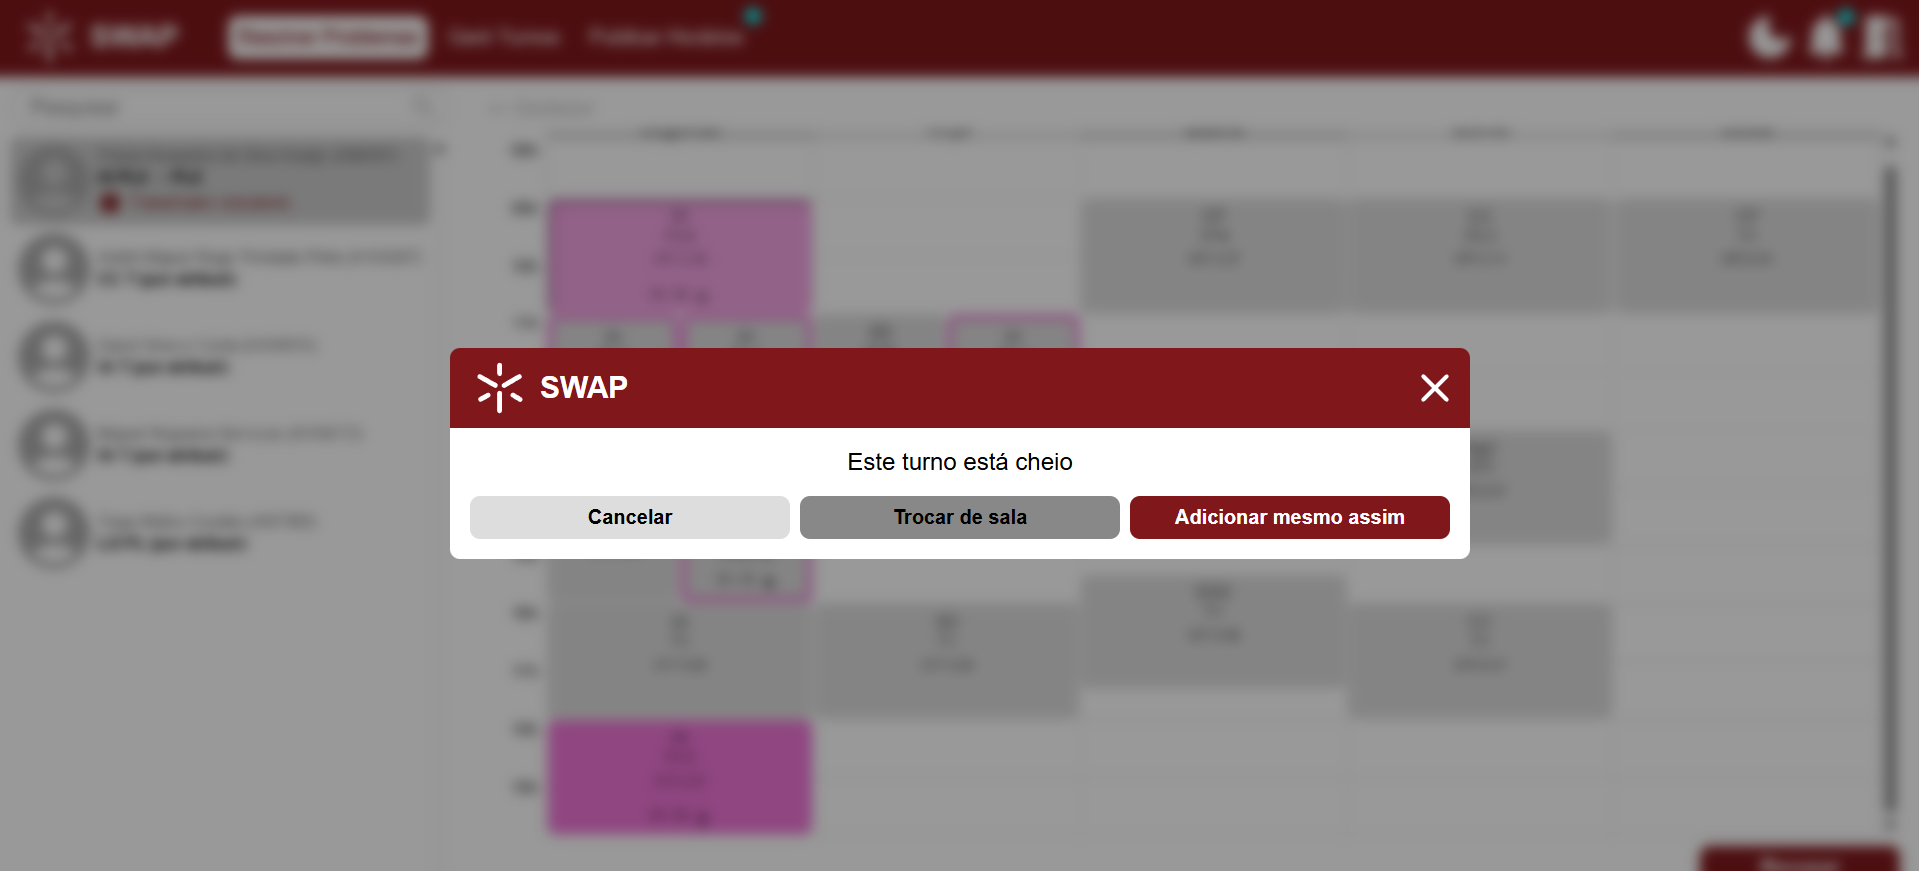
\includegraphics[width=0.8\textwidth]{res/manual/popup_turno_cheio.png}
    \caption{Popup que avisa que o turno ao qual se pretende adicionar um aluno está cheio.}
    \label{popup_turno_cheio}
\end{figure}

\textbf{- Realizar a troca de turno:}

Clicando então no turno pretendido, o aluno fica inscrito no mesmo de maneira provisória. Para fazer
com que esta mudança tenha efeito no horário do aluno, é necessário ir à página
``Publicar Horários'' e atualizar o horário dos alunos (figura \ref{publicar_horarios}).
Logicamente, o diretor de curso pode e deve atender a vários pedidos dos alunos e apenas publicar os
horários depois de concluir todas as alterações aos horários que desejava fazer.

\subsubsection{Outras funcionalidades}

\textbf{- Gerir um turno:}

O diretor de curso pode também, na página de gestão de um turno (figura \ref{gerir_turno}),
para além de consultar a lotação e trocar a sala de um turno, consultar e fazer a gestão dos
alunos inscritos no mesmo. Na lista de alunos do lado direito, é possível pesquisar por nome do
aluno, retirar um aluno do turno clicando no X, e adicionar um aluno no botão do canto superior
direito.

\begin{figure}[H]
    \centering
    \includegraphics[width=0.8\textwidth]{res/manual/gerir_turno_pesquisar_alunos.png}
    \caption{Pesquisa por alunos na página ``Gerir Turno''.}
    \label{gerir_turno_pesquisar}
\end{figure}

No diálogo para adicionar um novo aluno, é apresentada uma lista dos alunos inscritos na Unidade
Curricular a que o turno que se está a gerir pertence, com exceção dos alunos já inscritos no turno
a ser gerido. Também é possível procurar alunos nesta lista. Para adicionar um aluno desta lista ao
turno, clica-se no botão ‘+’ a si associado.

\begin{figure}[H]
    \centering
    \includegraphics[width=0.8\textwidth]{res/manual/adicionar_aluno.png}
    \caption{Diálogo para adicionar um aluno na página ``Gerir Turno''.}
    \label{adicionar_aluno}
\end{figure}

Para estas mudanças terem efeito, também é necessário publicar o horário, como descrito
anteriormente (figura \ref{publicar_horarios}).

\textbf{- Mudar para o modo escuro:}

Clicando no ícone de Lua no canto superior direito, o diretor de curso pode mudar a aplicação
para o modo escuro, que passa a ter um aspeto como o que se apresenta abaixo:

\begin{figure}[H]
    \centering
    \includegraphics[width=0.8\textwidth]{res/manual/modo_escuro_diretor.png}
    \caption{Exemplo de uma página no modo escuro.}
    \label{modo_escuro_diretor}
\end{figure}

Para voltar ao modo claro, é necessário clicar no botão de novo, que agora tem um ícone de Sol.

\textbf{- Terminar sessão:}

Para terminar a sua sessão, o diretor de curso deve clicar no botão com um ícone de porta no canto
superior direito da barra de navegação, voltando assim à página ``Iniciar Sessão''.

\subsection{Aluno}

\subsubsection{Cenário 4}

Para um aluno realizar as operações descritas no Cenário 4, ou seja, entrar na aplicação, consultar
o seu horário e enviar um pedido de troca de turno, os passos a efetuar são os seguintes:

\textbf{- Iniciar sessão com as suas credenciais:}

Para se autenticar, o aluno segue o mesmo processo que o diretor de curso na página
``Iniciar Sessão'' (figura \ref{pagina_login_vazia}).

\textbf{- Consultar o seu horário:}

Quando o aluno inicia a sua sessão, a primeira página que vê é a página do seu horário:

\begin{figure}[H]
    \centering
    \includegraphics[width=0.8\textwidth]{res/manual/pagina_o_meu_horario.png}
    \caption{Página ``O Meu Horário''.}
    \label{meu_horario}
\end{figure}

\textbf{- Procurar uma troca de turno:}

Supondo que, como descrito pelo cenário, o aluno pretende trocar os seus turnos de quinta-feira de
manhã para outros dias, o primeiro passo será clicar nos turnos em questão, neste caso, o CC - PL3,
que fará surgir o diálogo abaixo:

\begin{figure}[H]
    \centering
    \includegraphics[width=0.8\textwidth]{res/manual/popup_turno_meu_horario.png}
    \caption{Diálogo com informações de um turno.}
    \label{popup_turno}
\end{figure}

De seguida, o aluno clica no botão ``Procurar Troca'', que o leva para o seguinte ecrã:

\begin{figure}[H]
    \centering
    \includegraphics[width=0.8\textwidth]{res/manual/pagina_procura_troca_meu_horario.png}
    \caption{Troca de turno na página ``O meu Horário''.}
    \label{procura_troca}
\end{figure}

Aqui, o aluno pode ver o turno que pretende trocar, as opções de turnos para onde pode ir, as suas
capacidades, e o seu horário atual, de forma a poder ver com facilidade se a troca que deseja fazer
causará ou não conflitos no seu horário. Por exemplo, caso o aluno selecione trocar para o turno
CC - PL5, deparar-se-á com o diálogo abaixo:

\begin{figure}[H]
    \centering
    \includegraphics[width=0.8\textwidth]{res/manual/popup_pedir_troca.png}
    \caption{Pedido de confirmação de troca de turno.}
    \label{popup_pedir_troca}
\end{figure}

Clicando em ``Confirmar'', o pedido será enviado ao diretor de curso, e a seguinte mensagem de
confirmação aparecerá por cima do horário do aluno:

\begin{figure}[H]
    \centering
    \includegraphics[width=0.8\textwidth]{res/manual/toast_confirmacao_troca.png}
    \caption{Confirmação de sucesso na submissão de um pedido de troca de turno.}
    \label{toast_pedido_troca}
\end{figure}

\subsubsection{\emph{Outras funcionalidades}}

O aluno, para além do descrito acima, tem também as seguintes opções:

\textbf{- Ver o horário completo:}

Se o aluno, através da barra de navegação, for para a página ``Horário Completo'', pode ver o
horário de todos os turnos das Unidades Curriculares em que está inscrito, com destaque para os
turnos do seu horário. Para organizar esta grande quantidade de informação, o aluno pode, na barra
lateral, selecionar os turnos que pretende que lhe sejam apresentados:

\begin{figure}[H]
    \centering
    \includegraphics[width=0.8\textwidth]{res/manual/horario_completo.png}
    \caption{Página ``Horário completo''.}
    \label{horario_completo}
\end{figure}

\begin{figure}[H]
    \centering
    \includegraphics[width=0.8\textwidth]{res/manual/horario_completo_filtrado.png}
    \caption{Página ``Horário completo'' com alguns turnos por selecionar.}
    \label{horario_completo_filtrado}
\end{figure}

Esta página pode ser útil para alunos que desejam fazer mudanças ao seu horário mais complexas do
que a troca de um ou dois turnos. Deste modo, podem ver mais informação, e selecionar exatamente a
informação que desejam ver (o seu horário atual, os turnos que desejam, \ldots).

Nesta página também é possível clicar num turno para ver mais informações sobre o mesmo e procurar
uma troca, tal como na página ``O meu Horário''. Durante uma troca de turnos, diferentes turnos
são estilizados de diferente modo para realçar as opções de troca possíveis, o horário atual do
aluno, outros turnos visíveis, \emph{etc.}

\begin{figure}[H]
    \centering
    \includegraphics[width=0.8\textwidth]{res/manual/procura_troca_horario_completo.png}
    \caption{Procura de turno na página ``Horário Completo''.}
    \label{procura_troca_horario_completo}
\end{figure}

\textbf{- Ver o Histórico de Pedidos:}

O aluno tem também a possibilidade de consultar os pedidos de troca de turno que já realizou e o seu
estado (pendente, aceite ou rejeitado), navegando para a página ``Histórico de Pedidos'':

\begin{figure}[H]
    \centering
    \includegraphics[width=0.8\textwidth]{res/manual/historico_pedidos.png}
    \caption{Página ``Histórico de Pedidos'' com pedido pendente.}
    \label{historico_pedidos}
\end{figure}

\begin{figure}[H]
    \centering
    \includegraphics[width=0.8\textwidth]{res/manual/historico_pedidos_resolvido.png}
    \caption{Página ``Histórico de Pedidos'' com pedido aceite.}
    \label{historico_pedidos_resolvido}
\end{figure}

\textbf{- Ver as notificações:}

O aluno pode também ver as suas notificações, que correspondem a mudanças no seu horário, clicando
no botão com um ícone de sino no canto superior direito:

\begin{figure}[H]
    \centering
    \includegraphics[width=0.8\textwidth]{res/manual/notificacoes_aluno.png}
    \caption{Página ``Notificações do aluno''.}
    \label{notificacoes_aluno}
\end{figure}

\textbf{- Mudar para o modo escuro:}

Tal como o diretor de curso, o aluno pode também mudar a aplicação para o modo escuro (figura
\ref{modo_escuro_diretor}).

\textbf{Terminar sessão:}

Tal como o diretor de curso, o aluno termina sessão clicando no botão com um ícone de porta no
canto superior direito da barra de navegação, voltando assim à página ``Iniciar Sessão''.

\section{Acessibilidade}

Durante o processo de desenvolvimento da aplicação, foi feito algum esforço para a tornar acessível.

Em primeiro lugar, o código da aplicação tira proveito da semântica de várias \emph{tags} HTML
(\texttt{nav}, \texttt{li}, \texttt{button}, \ldots), pelo que se espera que leitores de ecrã sejam
capazes de compreender as páginas sem recurso a ARIA \emph{labels}, e oferecer uma boa experiência
de utilização a utilizadores com deficiências visuais. Para validar esta e outras hipóteses, a
extensão WAVE \cite{wave} e o programa Pa11y \cite{pa11y} foram utilizados para procurar diversos
problemas de acessibilidade, que o nosso grupo de trabalho procurou corrigir. Também no âmbito da
percetibilidade, garantiu-se que os rácios de contraste entre o fundo e texto dos componentes eram
aceitáveis, pelo menos no tema claro. No tema escuro, isto não se verifica, visto que a cor da
Universidade do Minho, utilizada em vários elementos da interface, não contrasta bem com tons
escuros. Mesmo assim, o utilizador tem a opção de utilizar o tema claro caso o necessite.

No âmbito da operabilidade, o nosso principal foco do foi o de garantir que era possível navegar
pelas várias páginas com o teclado de uma forma que faça sentido. A título de exemplo, é possível
fechar diálogos e \emph{toasts} com a tecla \texttt{Esc}, e é possível desfazer ações com
\texttt{Ctrl+Z}. Ademais, foi preciso especial cuidado nos horários para estes serem facilmente
navegáveis com a tecla \texttt{Tab}: como estes têm um \emph{layout} tabular, linha a linha, foi
preciso reajustar os valores de \texttt{tabindex} para garantir que os turnos eram visitados em
ordem cronológica. Também se garantiu que os elementos selecionáveis tinham a sua classe CSS
\texttt{:focus-visible} estilizada.

No entanto, o principal problema que a aplicação sofre é a falta de responsividade perante
diferentes tamanho de ecrã: são poucas as páginas e componentes que funcionam em ecrãs pequenos e
verticais como os dos \emph{smartphones}. Fazer as alterações necessárias ao \emph{layout} das
páginas para suportar variadíssimos tamanhos de ecrãs já envolveria bastante trabalho, mas também
aumentaria significativamente o número de testes que se teriam de fazer a cada página: cada página
teria de ser testada em vários navegadores e em vários tamanhos de ecrã, sendo que qualquer mudança
ao \emph{layout} envolveria refazer toda esta testagem. Devido ao tempo que isto consumiria, optámos
por dedicar mais tempo a melhorar a \emph{user experience} na aplicação, do que a a otimizar para
diversos tamanhos de ecrã. No entanto, no futuro, se esta aplicação fosse usada em produção,
\emph{layout} responsivo seria um das primeiras funcionalidades a ser implementada.

\section{Reflexão sobre a Aplicação}

Devido a falta de tempo, não foi possível avaliar a aplicação desenvolvida com utilizadores reais.
Mesmo assim, apresentam-se, nesta secção, alguns comentários pessoais do nosso grupo sobre a
aplicação final desenvolvida.

Em primeiro lugar, é necessário notar que a aplicação cumpre os requisitos propostos, permitindo ao
diretor de curso e aos alunos executar as ações nos cenários do enunciado do trabalho prático.
Ademais, é necessário considerar que o modelo Figma da interface previamente construído foi avaliado
de forma positiva, tanto heuristicamente como pela equipa docente. Visto que a aplicação
implementada seguiu este modelo do modo mais próximo possível, acredita-se que a aplicação também
providenciará uma boa experiência para o utilizador.

No entanto, surgiram alguns aspetos que podiam ser melhorados numa eventual próxima iteração no
desenvolvimento da aplicação. Em primeiro lugar, em páginas que dão a possibilidade ao utilizador de
desfazer uma ação, também é importante dar a possibilidade de refazer uma ação previamente desfeita,
algo que está em falta na aplicação desenvolvida. Ademais, na forma como as notificações são
geridas, a experiência do utilizador melhoraria se as notificações fossem automaticamente aceites
conforme as ações do utilizador. Por exemplo, se o diretor de curso visse o conteúdo de um pedido de
mudança de sala e alterasse a sala em que o turno é lecionado, a notificação deveria automaticamente
ser marcada como aceite. Estes pequenos detalhes são cruciais para assegurar uma boa experiência
de utilização e, apesar de poucos, acreditamos que há espaço para melhoria na aplicação
desenvolvida.

\section{Conclusão}

Em suma, ao longo deste semestre, foi levado a cabo o processo completo de desenvolvimento de uma
interface, partindo da sua modelação, passando pela sua implementação, e terminando na sua testagem
e avaliação. Em relação à segunda fase do trabalho prático, devido ao grande número de ferramentas
utilizado, foi possível aprender um pouco sobre diversos aspetos de desenvolvimento Web, apesar de
não ter sido possível aprofundar muito o nosso conhecimento em áreas específicas. Por muito que não
tenha sido possível realizar a fase da avaliação da aplicação com o detalhe que era desejado,
acreditamos que o produto desenvolvido não só cumpre os requisitos propostos, como também o faz
apresentando uma boa experiência de utilização.

\begingroup
\section{Bibliografia}
\renewcommand{\section}[2]{}

\begin{thebibliography}{9}
    \bibitem{vue}
        ``The Progressive JavaScript Framework''. Figma. Accessed: Apr. 30, 2025. [Online.]
        Available: \url{https://vuejs.org/}
    \bibitem{figma}
        ``Figma: Collaborative Interface Design Tool''. Figma. Accessed: Mar. 13, 2025. [Online.]
        Available: \url{https://www.figma.com/}
    \bibitem{typescript}
        ``TypeScript''. TypeScript. Accessed: Apr. 30, 2025. [Online.] Available:
        \url{https://www.typescriptlang.org/}
    \bibitem{blazor}
        `` Launch your idea to the web fast with Blazor''. Blazor. Accessed: Apr. 30, 2025.
        [Online.] Available: \url{https://dotnet.microsoft.com/en-us/apps/aspnet/web-apps/blazor}
    \bibitem{pinia}
        ``Pinia: The intuitive store for Vue.js''. Pinia. Accessed: Apr. 30, 2025. [Online.]
        Available: \url{https://pinia.vuejs.org/}
    \bibitem{pinia-persistent}
        ``Pinia Plugin Persistedstate: Configurable persistence of Pinia stores''.
        Pinia Plugin Persistedstate. Accessed: Apr. 30, 2025. [Online.] Available:
        \url{https://prazdevs.github.io/pinia-plugin-persistedstate/}
    \bibitem{json-server}
        ``json-server''. GitHub. Accessed: Apr. 24, 2025. [Online.] Available:
        \url{https://github.com/typicode/json-server}
    \bibitem{npm}
        ``NPM''. NPM. Accessed: Apr. 24, 2025. [Online.] Available: \url{https://www.npmjs.com/}
    \bibitem{eslint}
        ``ESLint''. ESLint. Apr. 24, 2025. [Online.] \url{https://eslint.org/}
    \bibitem{prettier}
        ``Prettier''. Prettier. Apr. 24, 2025. [Online.] \url{https://prettier.io/}
    \bibitem{wave}
        ``WAVE - Web Accessibility Evaluation Tool''. WAVE. Accessed: May 4, 2025. [Online.]
        Available: \url{https://wave.webaim.org/extension/}
    \bibitem{pa11y}
        ``Pa11y''. Pa11y. Accessed: May 4, 2025. [Online.] Available: \url{https://pa11y.org/}
\end{thebibliography}
\endgroup

\includepdf[pages=1,pagecommand=\section{Anexo -- Enunciado do Trabalho}\thispagestyle{empty}]
    {../Assignment.pdf}
\includepdf[pages=2-]{../Assignment.pdf}

\end{document}
